\documentclass[%
11pt,%
%oneside,%
twoside,%
%twocolumn,%
titlepage,%
%fleqn,%
%a4page,%
german,%
headsepline%
]{scrartcl}

%\usepackage{fancyhdr}
%\usepackage{scrpage}
\usepackage{lastpage}
\usepackage{geometry}
\usepackage{graphicx}
\usepackage[utf8]{inputenc}
\usepackage[ngerman]{babel}
\usepackage{lscape}
\usepackage[framemethod=TikZ]{mdframed}
\usepackage[most]{tcolorbox}
\usepackage{mymath}
\usepackage{units}
\usepackage{nicefrac}
\usepackage{pgf,tikz,pgfplots}
\pgfplotsset{compat=1.14}
\usepackage{mathrsfs}
\usetikzlibrary{arrows}
\usepackage{colortbl}
\usepackage{hhline}
\usepackage{multirow}
\usepackage[extendedchars]{grffile}
\usepackage{caption}
\usepackage{multicol}
\setlength{\columnsep}{1cm}
\usepackage{calc}
\usepackage{blindtext}
\usepackage{pdfpages}
\usepackage{hyperref}
%\usepackage{tikz-er2}
\usepackage{framed}
\usetikzlibrary{arrows}
\usetikzlibrary{positioning}
\usetikzlibrary{shadows}

\setlength{\parindent}{0pt}

\usepackage{marginnote}
\usepackage[]{qrcode}
\qrset{height=9ex}

%\usepackage{romannum}
\usepackage{longtable}
\usepackage{listings}
\usepackage{wrapfig}


% Command, um Tabellen-Spalten anzupassen
\newcommand{\spaltenheight}{\rule{0mm}{3ex}}
\newcommand{\spaltenwidth}{\rule{3cm}{0mm}}
\newcommand{\spaltensep}{\\[1ex]}
%\arrayrulecolor{darkgreen}
\doublerulesepcolor{white}
\definecolor{lightyellow}{rgb}{1,1,0.8}
\definecolor{Gray}{gray}{0.9}


% Pagestyle/Layout
%\geometry{a4paper , tmargin =2.5cm,	bmargin=3cm, lmargin =2.5cm,	rmargin =2.5cm,	headheight=3em, headsep=1em, footskip=1cm}
%\setlength{\parindent}{0pt} \setlength{\parskip}{1em}
%für TwoSide
%\lhead{\headmark\pagemark}
%\cehead{}
%\rehead{}
%\lohead{}
%\cohead{}
%\rohead{\headmark}
%für OneSide
%\ihead{}
%\chead{}
%\ohead{}
%\setheadsepline{0.5pt} % Linie zur Begrenzung
%\setfootsepline{0.5pt} % Linie zur Begrenzung
\pagestyle{headings} % gemachte Einstellungen anwenden


\subject{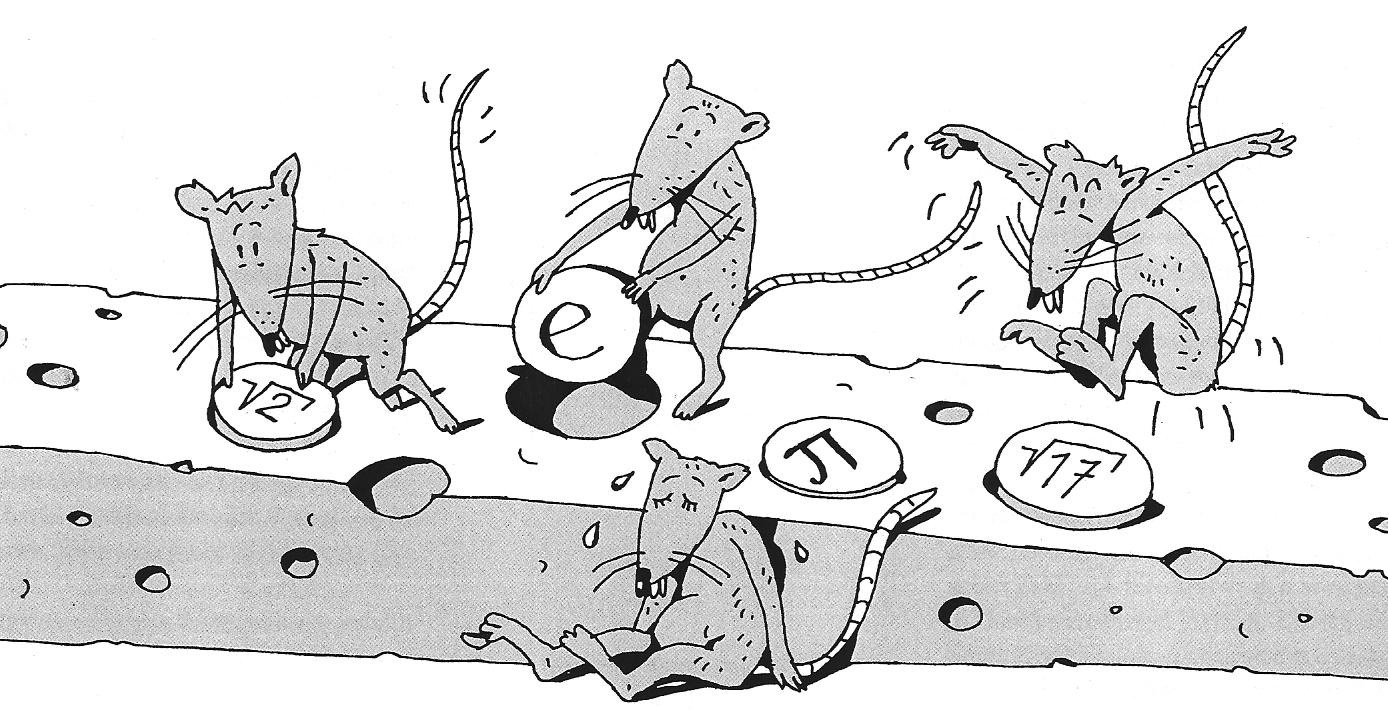
\includegraphics[width=0.618\textwidth]{pictures/irratzahlen}}
\title{Zahlen}
\subtitle{I like primes!}
\author{}
\date{}
%\lowertitleback{
%\includegraphics[height=1.1cm]{/Users/jormawassmer/Pictures/logokoeniz.jpg}%
%\copyright Jorma Wassmer
%1. Auflage, Februar 2011
%}


\begin{document}
\maketitle
\tableofcontents
%\thispagestyle{empty}
\cleardoublepage
%\setcounter{page}{1}

\section{Natürliche Zahlen}
\subsection{Historisches}
\begin{quote}
Alles ist Zahl.
\end{quote}

\begin{wrapfigure}{r}{0.382\textwidth}
\vspace{-22pt}
  \begin{center}
    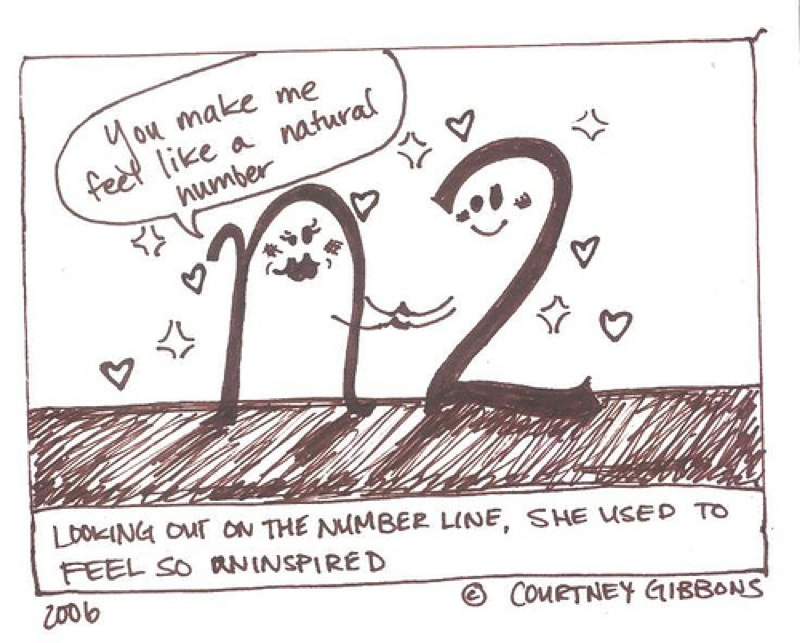
\includegraphics[width=0.38\textwidth]{pictures/zahln}
  \end{center}
%\caption{A gull}
\vspace{-22pt}
\end{wrapfigure}
Diese kurze, prägnante Aussage stammt von \textsc{Pythagoras}, dem berühmten griechischen Philosophen und Mathematiker, der um $\unit[550]{v.u.Z.}$ gelebt hat.

Die meisten schriftlichen Zeugnisse über \textsc{Pythagoras} und seine Anhänger gehen auf Darstellungen zurück, die mehr als $\unit[800]{Jahre}$ nach seinem Tod geschrieben und reichlich ausgeschmückt worden sind. \textsc{Pythagoras} gehört deshalb zu den rätselhaftesten Persönlichkeiten der Antike. Immerhin gilt seine Existenz als gesichert.

In jungen Jahren soll er sich auf Anraten von \textsc{Thales} ($\unit[624-546]{v.u.Z.}$) auf eine langjährige Studienreise nach Ägypten begeben haben, um dort die vorhandenen Wissensschätze zu studieren; vielleicht war er auch in Babylon. Der Zusammenhang der pythagoräischen Arithmetik mit der babylonischen legt jedenfalls eine solche Vermutung nahe. Nach \textsc{Pythagoras} sollte das menschliche Leben geordnet und harmonisch sein, wie es die Zahlenverhältnisse in der Natur offenbarten. Dieses Zahlenverständnis kommt im Satz \glqq Alles ist Zahl\grqq\ treffend zum Ausdruck und verdeutlicht, dass er und seine Schüler --- die nach ihm benannten Pythagoräer --- die Zahlen als eine, die gesamte Natur konstruierende Kraft betrachteten.

Kulturgeschichtlich blieben die Pythagoräer und ihre Schule bis weit über den Tod ihres Begründers bedeutsam. Sie prägten die Mathematik für Jahrhunderte.

\begin{quote}
Die natürlichen Zahlen hat Gott geschaffen, alles andere ist Menschenwerk.
\end{quote}
Dieses Zitat stammt von  \textsc{Leopold Kronecker} (1823--1891), ein Zahlentheoretiker und Analytiker. Er war einflussreicher Wegbegleiter des mathematischen Konstruktivimus, der nur mathematische Gegenstände gelten liess, deren Existenz durch explizite Konstruktion gesichert werden konnte. Sein Versuch, die Mathematik nur auf Grundlage der natürlichen Zahlen zu definieren, führte insbesondere zum Konflikt mit \textsc{Cantor} und dessen Mengenlehre, die dieser weitestgehend unkonstruktivistisch untersuchte.

\subsection{Die Menge der natürlichen Zahlen}

Die natürlichen Zahlen $\mathbb{N}$ sind die seit Alters her beim Zählen verwendeten Zahlen.
Mit ihnen kann man eine Menge durchnummerieren. Die natürlichen Zahlen haben einen Anfang, die $1$, aber kein Ende. Es gibt demnach unendlich viele dieser Zahlen. Ausserdem hat sich herausgestellt, dass die Menge $\mathbb{N}$ die kleinste Menge ist, die unendlich viele Elemente enthält (\textsc{Cantor}, Mengenlehre). Das Symbol für Unendlich ist eine liegende Acht, $\infty$.
\begin{bem}
Achtung: $\infty$ ist keine Zahl!
\end{bem}
Auf $\mathbb{N}$ können die Grundoperationen Addition und Multiplikation abgeschlossen durchgeführt werden, d.h. dass auch das Ergebnis einer solchen Operation wieder eine natürliche Zahl ist. Man sagt auch, die natürlichen Zahlen sind \textbf{abgeschlossen} bezüglich der Addition und Multiplikation.
Die Null gehört nicht zu den natürlichen Zahlen. Wird $\mathbb{N}$ aber mit der Zahl Null erweitert, schreibt man $\mathbb{N}_0$.
Zur Darstellung der natürlichen Zahlen eignet sich der \textbf{Zahlenstrahl}.
\begin{center}
\scalebox{1.3}{
\begin{tikzpicture}[line cap=round,line join=round,>=triangle 45,x=0.8cm,y=0.4cm]
\draw[->,color=black] (-3.68,0) -- (5.6,0);
\foreach \x in {-3,-2,-1,0,1,2,3,4,5}
\draw[shift={(\x,0)},color=black] (0pt,2pt) -- (0pt,-2pt) node[below] {\footnotesize $\x$};
\draw[color=black] (5.3,0.1) node [anchor=south west] {$\mR$};
%\draw[color=black] (0pt,-10pt) node[right] {\footnotesize $0$};
\clip(-3.68,-1.32) rectangle (5.36,1.56);
\end{tikzpicture}
}
\end{center}
Eine saubere Fundierung der natürlichen Zahlen gelang im $\unit[19.]{Jahrhundert}$. Ein bedeutender Beitrag dazu stammte von Cantor, dem die Einbindung des Unendlichen, $\infty$, gelang.
\marginnote{
\qrcode{
https://www.youtube.com/watch?v=qIfY1jMqjqY}
}
Er schuf mit der Mengenlehre ein Fundament, in dem einerseits die natürlichen Zahlen sicher eingebettet sind, aber auch der Begriff des Unendlichen nicht mit ihnen in Konflikt oder Widerspruch gerät.

\subsection{Primzahlen}

Unter den natürlichen Zahlen finden sich solche, die jedem Divisionsversuch mit einem natürlichen Divisor, der zwischen $1$ und der Zahl selbst liegt, widerstehen. Solche --- in diesem Sinne teilerlose --- Zahlen werden Primzahlen genannt.
\begin{cdef}[Primzahl]{}
Eine Zahl, die genau zwei verschiedene, natürliche Teiler hat, heisst \textbf{Primzahl}.
\end{cdef}
Somit gehören die Zahlen
$$2,3,5,7,11,13,17,19,23,\dots$$
zu den Primzahlen.
\begin{bem}
Beachte, dass $1$ per Definition keine Primzahl ist!
\end{bem}

Primzahlen sind die Bausteine der natürlichen Zahlen. Dies besagt der folgende und zugleich verblüffende Satz, den ich gerne als Satz der DNA der natürlichen Zahlen bezeichne.
\begin{csatz}[\glqq DNA der Zahlen\grqq]{}
Jede natürlich Zahl grösser $1$ lässt sich eindeutig als Produkt von Primzahlen darstellen.
\end{csatz}
\begin{proof}
Man kann beispielsweise einen Widerspruchsbeweis über die Existenz und Eindeutigkeit führen. Dazu braucht man die Tatsache, dass $\mathbb{N}$ wohlgeordnet ist. Die Details des Beweises sprengen den Rahmen dieser Veranstaltung.
\end{proof}
\begin{ueb}[Primfaktorzerlegung]
Zerlege die Zahlen $234600$ und $7571$ in ihre Primfaktoren.
\end{ueb}

\subsubsection{Etwas Zahlentheorie}

Als Bausteine der Zahlen scheinen die Primzahlen offensichtlich wichtig zu sein. Dies bemerkten schon die Griechen. Sie stellten vermutlich als erste die Frage nach deren Anzahl und deren Verteilung.

\subsubsection{Sieb von Eratosthenes}

Der alexandrinische Bibliothekar, Mathematiker und Geograph  \textsc{Eratosthenes} ($\unit[276-194]{v.u.Z.}$), der als erster einen ausgezeichneten Wert für den Umfang der Erde ermittelt hat, kannte bereits ein einfaches Verfahren, um die Primzahlen schrittweise aus der Reihe der natürlichen Zahlen heraus zu filtern (das Sieb des Eratosthenes). Um aber von einer grossen Zahl zu entscheiden, ob es sich um eine Primzahl handelt oder nicht, ist dieses Vorgehen nicht geeignet, da es langsam ist.

Betrachten wir die Primzahlen kleiner $100$:

\begin{quote}
2, 3, 5, 7, 11, 13, 17, 19, 23, 29, 31, 37, 41, 43, 47, 53, 59, 61, 67, 71, 73, 79, 83, 89, 97
\end{quote}

Auffallend ist, dass die Primzahlen scheinbar zufällig über $\mathbb{N}$ verteilt sind. Zudem gibt es Primzahlen, die sich als Paar um eine einzige Zahl schmiegen, wie zum Beispiel $11$ und $13$, $17$ und $19$, $29$ und $31$ oder $59$ und $61$. Die von einem solchen \textbf{Primzahlzwilling} eingeschlossene Zahl besitzt immer viele Teiler, auf jeden Fall den Teiler $6$.

\begin{ueb}[Primzahlzwillinge]
Beweise, dass die Zahl zwischen einem Primzahlzwilling, $(p|p+2)$ mit $p$, $p+2$ beide prim, durch $6$ teilbar ist.
\end{ueb}

Die Lücken, das heisst die Anzahl der nichtprimen Zahlen zwischen zwei Primzahlen, sind in der Reihe der natürlichen Zahlen ganz verschieden gross. Je weiter in der Zahlenreihe fortgeschritten wird, um so grössere, derartige Lücken --- nebst den kleinsten --- treten auf.

\subsubsection{Dichte von Primzahlen}

Deutlich ist, dass die Primzahlen im allgemeinen mit wachsenden Zahlenwerten weniger häufig auftreten. Aber auch diese Gesetzmässigkeit wird durchbrochen. So finden wir in den ersten Hunderter-Blöcken die folgenden Anzahlen Primzahlen:\\
\begin{center}
\begin{tabular}{rrr}
\rowcolor{Gray}\spaltenheight $1$ bis $100$ & $101$ bis $200$ & $201$ bis $300$\spaltensep
\rowcolor{lightyellow}\spaltenheight $25$ & $21$ & $16$\spaltensep
\rowcolor{Gray}\spaltenheight $301$ bis $400$ & $401$ bis $500$ & $501$ bis $600$\spaltensep
\rowcolor{lightyellow}\spaltenheight $16$ & $17$ & $14$\spaltensep
\rowcolor{Gray}\spaltenheight $601$ bis $700$ & $701$ bis $800$ & $801$ bis $900$\spaltensep
\rowcolor{lightyellow}\spaltenheight $16$ & $14$ & $15$\spaltensep
\rowcolor{Gray}\spaltenheight $901$ bis $1000$ & &\spaltensep
\rowcolor{lightyellow}\spaltenheight $14$ & &\spaltensep
\end{tabular}
\end{center}
Das erste Tausend weist also $168$ Primzahlen auf, was etwa $\nicefrac{1}{6}$ aller natürlichen Zahlen dieses Intervalls entspricht. In den ersten $3000$ finden sich etwa $\nicefrac{1}{7}$, und unter den ersten $10\,000$ treffen wir auf rund $\nicefrac{1}{8}$. Die Dichte nimmt also scheinbar ab.
\marginnote{
\qrcode{
https://www.youtube.com/watch?v=Lg9GPyNOmSE}
}
Ist die Menge der Primzahlen also endlich? Gibt es eine grösste Primzahl?
Der \emph{indirekte} Beweis der Antwort auf diese Frage, lieferte schon \textsc{Euklid}\footnote{griechischer Mathematiker um $\unit[350]{v.u.Z.}$.}
Der Beweis des Satzes, dass unendlich viele Primzahlen existieren, ist bis heute ein wunderbares Beispiel logischer Eleganz.
 
\begin{ueb}[unendlich viele Primzahlen]
    Zeige, dass es unendlich viele Primzahlen gibt.
\end{ueb}
 
\begin{figure}
\begin{center}
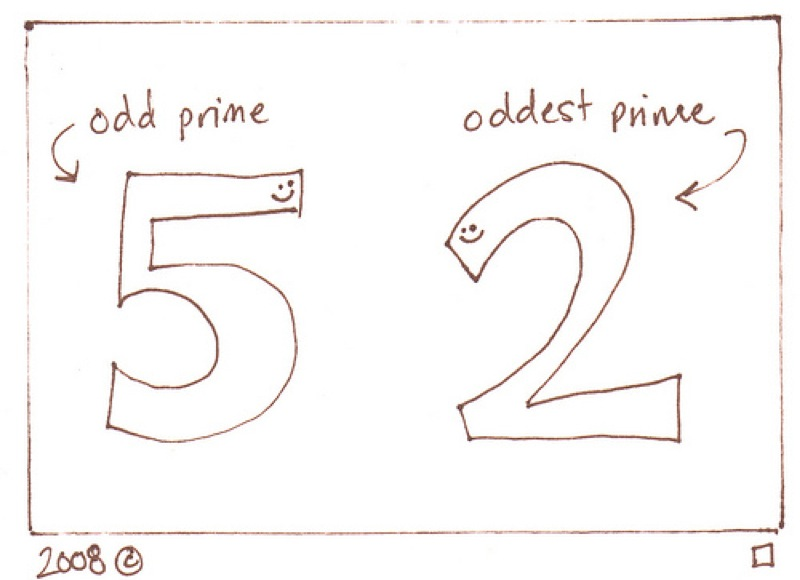
\includegraphics[width=0.3828\textwidth]{pictures/primzahl}
\caption{Seltsamste Primzahl}
\end{center}
\end{figure}
 
\subsubsection{Die Goldbach'sche Vermutung}
Ein Beispiel für eine einfach gestellte Vermutung zu Primzahlen, von der man bis heute (\the\year) nicht weiss, ob sie war ist oder nicht, ist die \textbf{Goldbach'sche Vermutung}: Jede gerade, natürliche Zahl grösser als $3$ die Summe zweier Primzahlen ist. Also zum Beispiel $4=2+2, 6=3+3, 8=3+5$ etc. Manche geraden Zahlen lassen sich sogar auf mehrere Arten als Summe zweier Primzahlen darstellen; beispielsweise ist $10=3+7=5+5$ oder $20=7+13=3+17$. Es wird vermutet, dass die Goldbach'sche Vermutung wahr ist, aber bewiesen wurde sie bis heute nicht. Jedoch wurde eine ähnliche Aussage über ungerade Zahlen --- nämlich dass genügend grosse ungerade Zahlen sich stets als Summe von $3$ Primzahlen schreiben lassen --- 1937 von \textsc{Ivan Vinogradov} bewiesen.
 
\subsubsection{Der grosse Satz von Fermat}
 
Ein um die Jahrtausendwende gelöstes zahlentheoretisches Problem, das sogar in der Presse seinen Niederschlag fand, ist der grosse Satz von Fermat.
\begin{csatz}[Grosser Fermat'scher Satz]{}
Für $,x,y,z,n\in\mathbb{N}$ mit $n>2$, $y$, $z$ und $n>2$ ist Gleichung
$$x^n+y^n=z^n$$
nicht erfüllbar.
\end{csatz}

\textsc{Fermat}\footnote{französischer Mathematiker (1601--1665)} selbst hinterliess auf dem Blattrand einer Manuskriptseite die Notiz:
\begin{quote}
    Wenn $n$ eine Zahl grösser als $2$ bedeutet, so gibt es keine positiven ganzen Zahlen $a$, $b$ und $c$, so dass $a^n+b^n=c^n$ wäre. Ich habe dafür einen wahrhaft wundervollen Beweis gefunden, der aber auf diesem Rande keinen Platz findet!
\end{quote}

\begin{bem}
    Für $n=2$ entspricht die oben genannte Gleichung dem Satz des Pythagoras, und der hat natürlich Lösungen. Man spricht in diesem Zusammenhang von \textsc{pythagoräischen Zahlentripeln}.
\end{bem}

\subsubsection{Fermat'sche Zahlen}
Der Zahlentheoretiker \textsc{Fermat} irrte hingegen sicher als er behauptete, dass jede Zahl der Form
$$2^a+1$$
dann eine Primzahl darstelle, wenn $a$ selbst eine Zweierpotenz sei. Und in der Tat ergeben sich für $a=2^0,2^1,2^2,2^3$ und $2^4$ die Primzahlen $3,5,17,257$ und $65537$. Dass die Formel aber bereits für $a=2^5$ eine Zahl\footnote{$2^{2^5}+1=4\,294\,967\,297=641\cdot6\,700\,417$} liefert, die nicht mehr prim ist, war Fermat merkwürdigerweise entgangen. Der grosse Basler Mathematiker \textsc{Leonard Euler}\footnote{Schweizer Mathematiker (1707--1783)} deckte den Fehler 1739 auf. Dass die von Fermat kreierten Zahlen
$2^{2^n}+1$ mit $n\in\mathbb{N}$, die so genannten \textsc{Fermat'schen Zahlen}, dennoch interessante Eigenschaften und verblüffende Zusammenhänge --- unter anderem zur Geometrie --- aufweisen, stellte ein anderer grosser Mathematiker fest. Im Jahre 1796 befasste sich  \textsc{Carl Friedrich Gauss}\footnote{Deutscher Mathematiker (1777--1855)}, damals 19-jährig, mit dem alten, in die klassische Zeit Euklids zurückführenden Problem der Konstruktion der regulären Polygone mit Zirkel und Lineal. In seinem berühmten Werk \emph{disquisitiones arithmeticae} legte \textsc{Gauss} die allgemeine Lösung der Aufgabe dar. Er konnte als erster zeigen, dass alle regulären Vielecke, deren Seitenzahl $p$ prim ist, dann und nur dann mit Zirkel und Lineal konstruierbar sind, wenn $p$ von der Form $2^{2^n}+1$ ist. Dieses $p$ gehört also, wie bereits erwähnt, zu den Fermat'schen Zahlen.

\subsubsection{Primzahlen im Internet}

Die Suche nach schnellen Verfahren zum Auffinden von Primzahlen dauert bis zum heutigen Tag an; und das nicht nur auf Grund des Reizes, den sie seit jeher auf die Menschen ausgeübt haben. Über zweitausend Jahre lang wusste man keinen praktischen Nutzen aus dem Wissen über die Primzahlen zu ziehen. Dies änderte sich allerdings schlagartig mit dem Aufkommen des elektronischen Datenverkehrs, als Primzahlen zum Verschlüsseln von Informationen eine zentrale Rolle zu spielen begannen (\textbf{Kryptographie}).

Die Güte einer Geheimsprache besteht einerseits darin, Botschaften ohne grossen Aufwand in Geheimschrift umschreiben (chiffrieren) zu können, andererseits darin, die Schwierigkeit für Uneingeweihte eine geheime Botschaft zu knacken (dechiffrieren), ins Unermessliche zu steigern. Solch asymmetrische Eigenschaften trifft man beim Rechnen mit Primzahlen an:
\begin{quote}
Es ist relativ einfach, das Produkt von zwei grossen Primzahlen zu berechnen, aber nahezu unmöglich, dieses Produkt wieder in seine Faktoren zu zerlegen.
\end{quote}
Das Verschlüsseln einer Botschaft läuft heute tatsächlich auf die Multiplikation zweier sehr grosser Primzahlen hinaus, während das Entschlüsseln im Wesentlichen aus dem Faktorisieren dieses Produkts besteht (ohne Kenntnis einer der beiden Faktoren ein praktisch aussichtsloses Unterfangen).

Bis heute hat man noch keinen schnellen Algorithmus zur Faktorisierung eines Produkts zweier grosser Zahlen gefunden. Ja, man weiss sogar nicht einmal, ob ein solcher überhaupt existiert. Gelänge es aber, einen Algorithmus zu finden, der eine schnelle Faktorzerlegung einer Zahl ermöglichen würde, so wöre unsere auf Diskretion und Geheimhaltung bedachte Kommunikationsgesellschaft nicht mehr in ihrer aktuellen Form denkbar. Denn alle Systeme, die auf Transaktionen sensibler Daten angewiesen sind --- wie Kreditkarten-, Telekommunikations- und nachrichtendienstliche System ---, werden durch Primzahlprodukte geschützt.

\subsection{Übungen zu $\mathbb{N}$ und Primzahlen}

\begin{ueb}[Primzahlformeln]
Was taugen die folgenden Formeln als Primzahlerzeuger? Dabei steht stets $p$ für eine Primzahl und $n$ für eine natürliche Zahl.

\begin{center}
    \begin{tabular}{ll}
        $z=2^p-1$ & $z=2^p+1$\\
        $z=n^2-79n+1601$ & $z=n^2-n+41$
    \end{tabular}
\end{center}
\end{ueb}

\begin{ueb}[Goldbach]
Wähle $5$ gerade Zahlen zwischen $3$ und $1000$. Versuche jeder dieser Zahlen als Summe von zwei Primzahlen darzustellen (Stichwort Goldbach'sche Vermutung).
\end{ueb}

\begin{ueb}[Zwillinge und Drillinge]
Sind $p$ und $p+2$ beides Primzahlen, so sprechen wir von \textbf{Primzahlzwillingen}.
\begin{enumeratea}
    \item Suche einige Primzahlzwillinge. Wie viele gibt es?
    \item Zeige, dass die zwischen einem Primzahlzwilling \glqq eingeklemmte\grqq{} Zahl sicher durch $6$teilbar ist.
    \item Suche Primzahldrillinge $p$, $p+2$, $p+4$. Wie viele gibt es?
\end{enumeratea}
\end{ueb}

\begin{figure}
    \begin{center}
        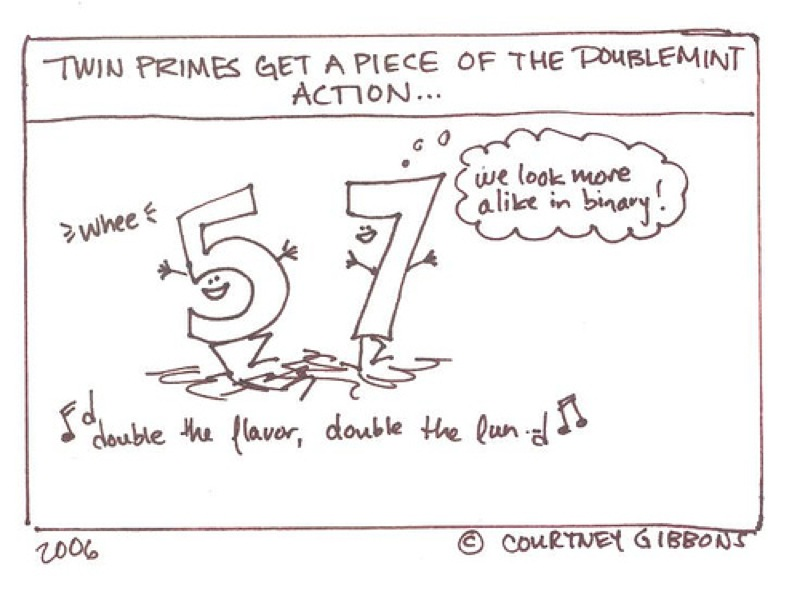
\includegraphics[width=0.382\textwidth]{pictures/primzahlzwillinge}
        \caption{Primzahlzwillinge}
    \end{center}
\end{figure}

\begin{ueb}[Primzahllücken]
Es gibt Primzahllücken beliebiger Grösse.
\begin{enumeratea}
    \item Betrachte die Zahl
    $$z=1\cdot2\cdot3\cdot4\cdot5\cdot6=6!$$
    und deren Nachfolger $6!+1$, $6!+2$, $6!+3$,\dots. Welche Nachfolger von $z$ sind keine Primzahlen?
    \item Betrachte die Zahl $50!$ und $1001!$ mit deren Nachfolgern. Welche Nachfolger sind sicher keine Primzahlen?
    \item $n!+1$ kann prim sein oder nicht. Suche Beispiele für beide Fälle.
\end{enumeratea}
\end{ueb}

\begin{ueb}[teilen]
Eine dreistellige Zahl wird zweimal hintereinander geschrieben, so dass eine sechsstellige Zahl entsteht. Diese Zahl wird anschliessend der Reihe nach durch $7$, durch $11$ und durch $13$ dividiert. Vermutung?
\end{ueb}

\begin{ueb}[Vierfache]
Zeige, dass die Summe von vier aufeinander folgenden natürlichen Zahlen niemals ein Vielfaches von $4$ sein kann.
\end{ueb}

\begin{ueb}[Vierersumme]
Vier aufeinander folgende natürliche Zahlen werden miteinander multipliziert und zum Produkt $1$ addiert.
\begin{enumeratea}
    \item Stelle einige konkrete Berechnungen an.
    \item Stelle eine Vermutung auf.
    \item Versuche, diese Vermutung zu beweisen.
\end{enumeratea}
\end{ueb}

\begin{ueb}[Quadratzahlen]
Suche Quadratzahlen, welche bei der Division durch $3$ den Rest $2$ lassen. Solltest du keine derartige Zahl finden, so versuche zu beweisen, dass es keine Quadratzahl gibt, die bei der Division durch $3$ den Rest $2$ lässt.
\end{ueb}

\subsection{ggT und kgV}
Primfaktorzerlegungen spielen auch beim Bestimmen des ggT (grösster gemeinsamer Teiler) und des kgV (kleinstes gemeinsames Vielfaches) zweier natürlicher Zahlen $a$ und $b$ eine wichtige Rolle.

\begin{ueb}[gcd and lcm]
Bestimme das kgV und den ggT der Zahlen $153900$ und $180600$.
\end{ueb}

\subsubsection{Euklid'scher Algorithmus}

Um den ggT zweier Zahlen $a$ und $b$ zu finden, gelangt man häufig mit dem \textsc{Euklid'schen Algorithmus} am schnellsten zum Ziel. Als Beispiel betrachten wir nochmals die beiden Zahlen $153900$ und $180600$, dividieren zuerst die grössere durch die kleinere und bestimmen danach den Rest, der entsteht.
\marginnote{
\qrcode{
https://www.youtube.com/watch?v=m8_OtbfpBnY}
}
In einem zweiten Schritt wird die kleinere Zahl durch den erhaltenen Rest geteilt und der dadurch resultierende neue Rest bestimmt, etc\dots.

Zwischen dem ggT und dem kgV besteht der folgende Zusammenhang.

\begin{csatz}[Produktsatz]{}
$$a\cdot b=\ggT(a,b)\cdot\kgV(a,b)$$
\end{csatz}

\begin{proof}
Bestätige die Richtigkeit des Satzes durch ein selbst gewähltes Beispiel.
\end{proof}

\begin{ueb}[Euklid'scher Algorithmus]
Bestimme den ggT und das kgV der Zahlen $5544$ und $4410$ mit dem euklidschen Algorithmus und dem letzten Satz.
\end{ueb}

\clearpage

\section{Die ganzen Zahlen}
\subsection{Die negativen Zahlen}

\subsubsection{Historisches}

\begin{wrapfigure}{r}{0.382\textwidth}
\vspace{-22pt}
  \begin{center}
    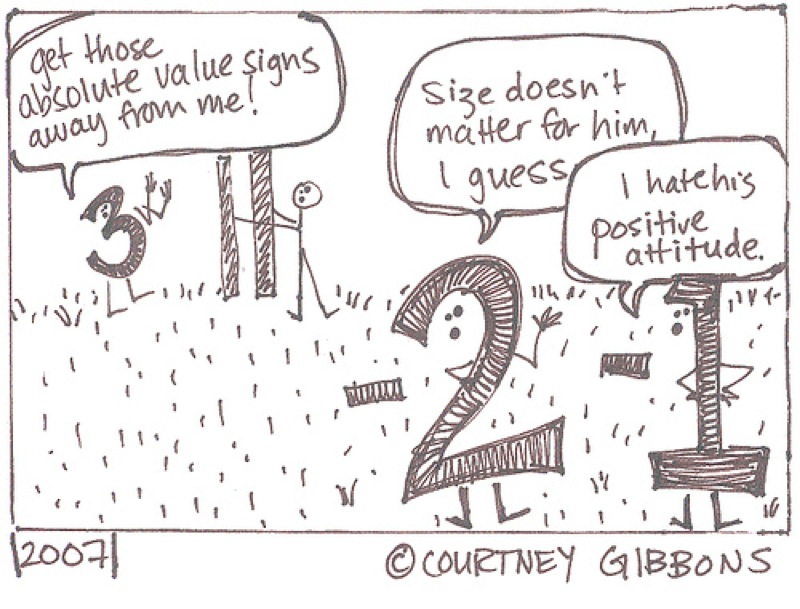
\includegraphics[width=0.38\textwidth]{pictures/negative}
  \end{center}
%\caption{Positive Attitude}
\vspace{-22pt}
\end{wrapfigure}
In unserer westlichen, von der griechischen Denkweise durchdrungenen Welt, bestand lange Zeit kein Anlass, die negativen Zahlen einzuführen. Solche Zahlen können in der Natur nicht gefunden werden. Zahlen dienten bis ins späte Mittelalter in Europa lediglich dazu, Abmessungen (Längen, Flächen- und Volumeninhalte) oder eine Anzahl von Gegenständen anzugeben.

Der indische Mathematiker und Astronom \textsc{Brahmagupta} (598-630) erkannte als einer der ersten das Wechselspiel von Zahlzeichen, indem er Regeln für das Teilen von Zahlen aufstellte: \glqq Positiv geteilt durch positiv oder negativ geteilt durch
negativ gibt positiv. Positiv geteilt durch negativ oder negativ geteilt durch positiv gibt negativ.\grqq Das könnte als Ursprung dessen bezeichnet werden, was wir heute \emph{Algebra} nennen. 

Der griechische Mathematiker \textsc{Diophant} (zwischen 100 v.u.Z. und 350 n.u.Z.) untersuchte zwar in seinem Werk \emph{Arithmetica} die Lösungen von Gleichungen. Eine Gleichung der Art
$$4x + 20 = 0$$
bezeichnete er aber als absurd. Negative Lösungen von Gleichungen wurden als bedeutungslos angeschaut.

Erst \textsc{Fibonacci} (1180-1241) erlaubte in seiner Finanzmathematik negative Zahlen und interpretierte sie korrekterweise als Schulden.

\subsubsection{Die Geschichte der Null}
Ein ähnlich schwieriger Stand wie die negativen Zahlen hatte die Zahl Null, die in Europa auf Ablehnung und
Unverständnis stiess: Null wurde mit nichts gleichgesetzt.

Im Anhang \ref{ap:null} ist ein Artikel von \textsc{Herbert Cerutti} abgedruckt, der im Februar 2002 im NZZ-Folio \emph{Total Digital} erschienen ist.

\newpage

\section{Rationale Zahlen}
\subsection{Normalbrüche}
\begin{wrapfigure}{r}{0.382\textwidth}
\vspace{-22pt}
  \begin{center}
    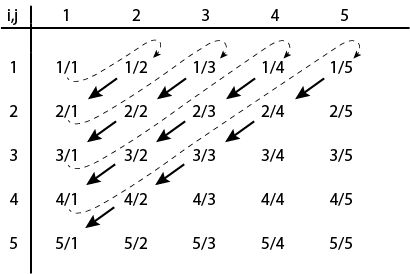
\includegraphics[width=0.38\textwidth]{pictures/Cantor}
  \end{center}
%\caption{Positive Attitude}
\vspace{-22pt}
\end{wrapfigure}
In der Menge der ganzen Zahlen $\mathbb{Z}$ kann die Division nicht immer
ausgeführt werden.
\bsp Die Rechnung $\,8\div 2\,$ liefert zwar wieder ein Element aus $\mathbb{Z}$ als Lösung (nämlich 4), aber $\;8\div 3\,$ ist in $\mathbb{Z}$ nicht mehr lösbar, denn $\,\frac{8}{3}=2.\overline{6}\notin\mathbb{Z}$. 
Wir suchen deshalb eine möglichst einfache Menge, welche die ganzen Zahlen enthält und welche die Division uneingeschränkt zulässt (ausser der Division durch 0, natürlich!).
Dies wird durch die Menge der rationalen Zahlen
$$\mathbb{Q} = \setm{\frac{p}{q}}{p\in\mathbb{Z},\,q\in\mathbb{N}}$$
gewährleistet. Dabei wird $p$ als Zähler und $q$ als Nenner des \textit{Normalbruchs} $\dfrac{p}{q}$
bezeichnet.

\subsection{Historisches}

Im Gegensatz zu den ganzen Zahlen tauchen die Bruchzahlen in der Geschichte schon sehr früh auf. Die ältesten wurden in summerischen und ägyptischen Texten gefunden. Die Ägypter kannten und benutzten sogenannte \textbf{Stammbrüche}, also Brüche, deren Zähler 1 ist. Alle anderen Brüche wurden als Summe von verschiedenen Stammbrüchen geschrieben. 

\begin{ueb}[Stammbrüche]
Stelle den Bruch $\frac{3}{4}$ auf mindestens zwei verschiedene Arten als Summe von verschiedenen Stammbrüchen dar.
\end{ueb}

\subsection{Dezimalbrüche}

Dezimalbrüche können in zwei Kategorien eingeteilt werden: Dezimalbrüche 
\begin{itemize}
	\item mit periodischer Dezimalbruchentwicklung (z.B. $1.5$ oder $3.5\overline{12}$)
	\item ohne periodische Dezimalbruchentwicklung (z.B. $0.10100100010\dots$)
\end{itemize}

\begin{bem}
Dezimalbrüche mit abbrechender Dezimalbruchentwicklung können unter der Menge Dezimalbrüche mit periodischer Dezimalbruchentwicklung subsummiert werden.
\marginnote{
\qrcode{
https://www.youtube.com/watch?v=GBgXSkXRu0g}
}
Zum Beispiel kann der abbrechende Dezimalbruch 1.5 auch als periodischer geschrieben werden, nämlich\dots
\end{bem}

\begin{csatz}[Dezimaldarstellung rationaler Zahlen]{}
Jeder Normalbruch lässt sich in Form eines periodischen Dezimalbruchs schreiben, und umgekehrt.
\end{csatz}

Um diesen Satz zu beweisen muss man zwei Dinge tun: Man muss zeigen, dass
\begin{itemize}
	\item jeder Normalbruch in einen periodischen Dezimalbruch und
	\item jeder periodische Dezimalbruch in einen Normalbruch umgewandelt werden kann.
\end{itemize}

Im Folgenden soll das Verfahren zur Umwandlung an ein paar Beispielen erläutert werden.

\subsection{Gedanken zu rationalen Zahlen}

\begin{ueb}[abbrechende rationale Zahlen]
Wie muss der Nenner eines Bruches beschaffen sein, damit die Dezimalbruchdarstellung abbrechend ist?
\end{ueb}

\begin{ueb}[Periodenlänge]
Behauptung: Die Periodenlänge eines Bruches
$$\frac{1}{q}$$
wird nie länger als $q-1$.
	\begin{enumeratea}
	  \item Warum ist dem so? Rechne Beispiele durch.
	  \item Betrachte die Periodenlängen von $\ \frac{1}{p}\,$ ($p$ prim). Kannst du diese Behauptung noch etwas präzisieren?
	\end{enumeratea}
\end{ueb}

\begin{ueb}[ein Siebtel]
Die Periode von
$$\frac{1}{7}$$
ist $0.142857$. Multipliziere diese Zahl mit $2,3,\dots$.
	\begin{enumeratea}
	  \item Was erkennst du? Kannst du dieses Muster erklären?
	  \item Bei der Multiplikation mit $7$ verschwindet dieses Muster. Warum?
	\end{enumeratea} 
\end{ueb}

\begin{ueb}

    \begin{enumerate}[a)]
        \item Verwandle den Bruch $\frac{3}{11}$ in eine Dezimalzahl.
        \item Bestimme den Bruch zur rationalen Zahl $0.1\overline{32}$.
    \end{enumerate}
\end{ueb}

\section{Reelle Zahlen}

Es scheint, als sei die Zahlengerade durch die \glqq überall dicht\grqq\
liegenden rationalen Zahlen lückenlos besetzt, da sich zwischen zwei
noch so nahe beieinander liegenden rationalen Zahlen immer noch unendlich viele andere rationale Zahlen befinden. Diese Ansicht ist
falsch! Es gibt noch Lücken, sogar mehr als einem lieb ist.
\subsection{Die Entdeckung der irrationalen Zahlen}
\begin{figure}
  \begin{center}
    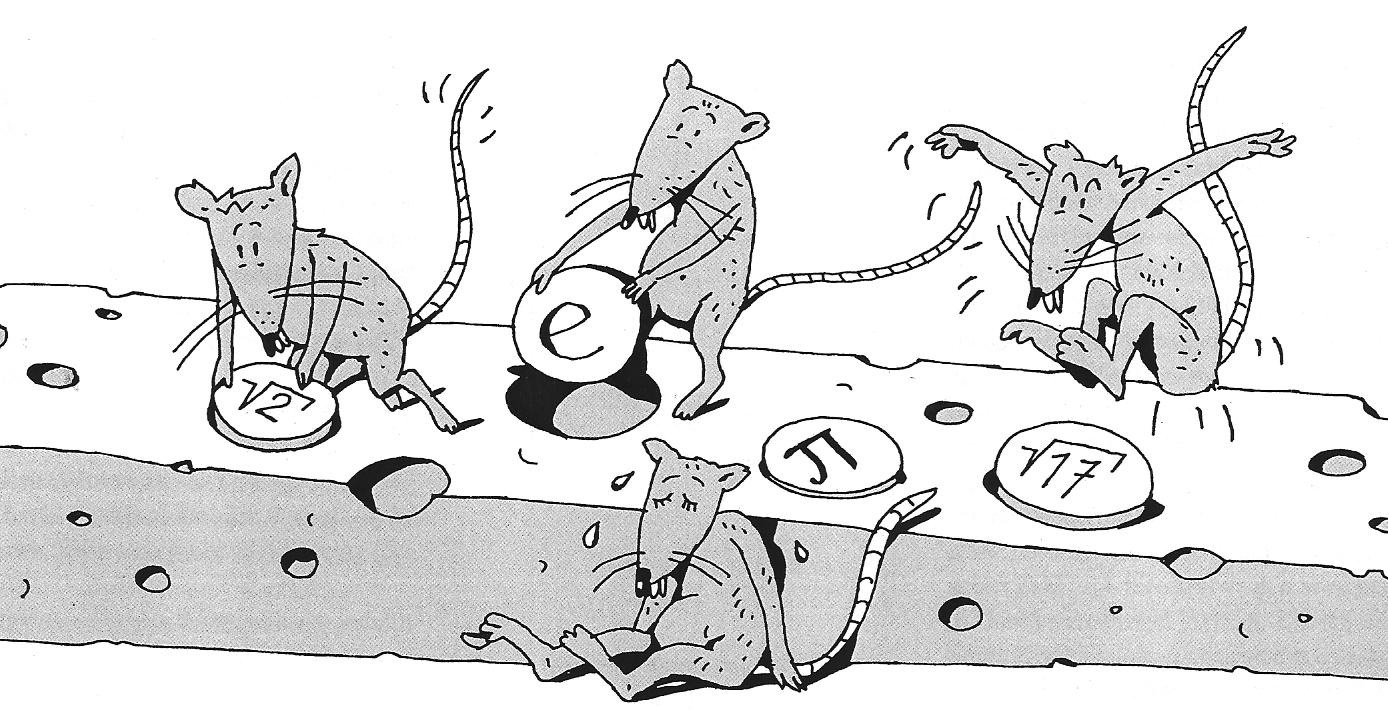
\includegraphics[width=0.382\textwidth]{pictures/irratzahlen}\hspace{2cm}
    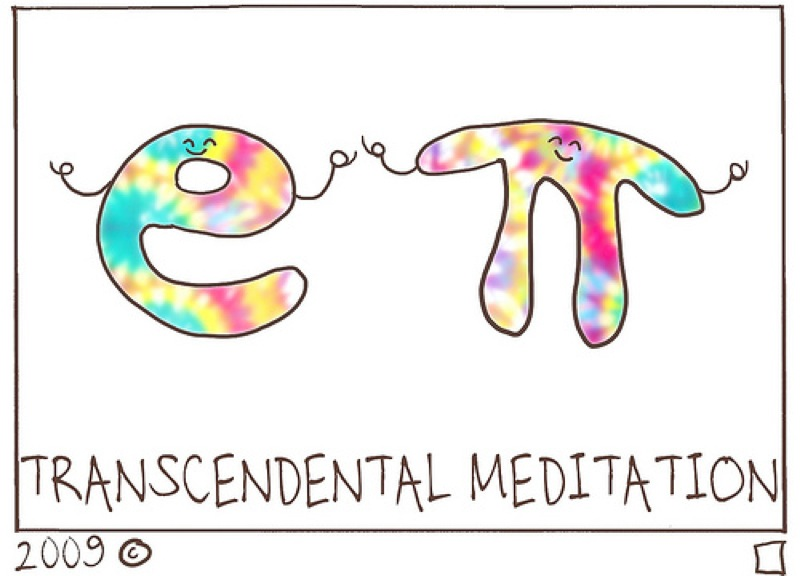
\includegraphics[width=0.382\textwidth]{pictures/transzendent}
  \end{center}
\caption{irrats and transcendents}
\end{figure}
In der goldenen Ära Griechenlands (bis ca.\ 400 v.u.Z.) galten unter den Gelehrten die natürlichen Zahlen und die Lehre ihrer Verhältnisse als das Mass aller Dinge. Die
Entdeckung von inkommensurablen Längen bedrohte deshalb ihr Bild
einer auf ganzzahligen Verhältnissen beruhenden Welt und riss eine
grosse Kluft zwischen die Arithmetik, die diese seltsamen \emph{irrationalen Zahlen} erschaffen konnte, und die Geometrie, die sie
nicht messen konnte. Eine dieser Zahlen, die nicht durch ein
Verhältnis zweier Zahlen ausgedrückt werden kann, ist $\sqrt{2}$.

\begin{proof}[Beweis]
Indirekter
\marginnote{
\qrcode{
https://www.youtube.com/watch?v=_ONbuGauF9I}
}
Beweis.
\end{proof}

Die irrationalen Zahlen können, da sie nicht messbar sind, nicht durch einen Bruch, das heisst also auch nicht durch einen (endlichen oder unendlichen periodischen) Dezimalbruch beschrieben
werden. Es muss sich also um unendliche nichtperiodische Dezimalbrüche handeln. Sie bilden zusammen mit den rationalen Zahlen die Menge der \textbf{reellen Zahlen}, $\mathbb{R}$. 

Neben den Wurzelzahlen $\sqrt{2}=1.41421\dots$, $\sqrt{3}=1.73205\dots$ etc.\ gehören Zahlen wie \textbf{Pi} $\pi=3.14159\dots$, die \textbf{Euler'sche Zahl} $\mathrm{e}=2.71828\dots$ und die Zahl des \textbf{goldenen Schnitts} $\Phi=1.61803\dots$
zu den berühmtesten irrationalen Zahlen des Altertums.

\begin{bem}
Die reellen Zahlen werden manchmal auch in zwei andere Mengen
aufgeteilt: In die \textbf{algebraischen}, die als Nullstellen von
Polynomen mit ganzzahligen Koeffizienten aufgefasst werden können, also im Wesentlichen Wurzelausdrücke, und in die
\textbf{transzendenten Zahlen}, das sind alle anderen. Während zum Ersteren die Zahl $\sqrt{2}$ und die des goldenen Schnitts $\phi$ gehören, sind die Zahlen $\pi$ und $\mathrm{e}$ transzendente Zahlen.
\end{bem}

\clearpage

\section{Dies \&\ Das zu Zahlenmengen}

\begin{ueb}[Klassifizieren]
Zu welcher kleinstmöglichen Zahlenmenge ($\mathbb{N}$, $\mathbb{Z}$, $\mathbb{Q}$ und $\mathbb{R}$) gehören die folgenden Zahlen:

\begin{minipage}{0.45\textwidth}
\begin{enumeratea}
\item $-5$
\item $4.\overline{7}$
\item $-\frac{5}{3}$
\item $5.155155515555\dots$
\end{enumeratea}
\end{minipage}
\begin{minipage}{0.4\textwidth}
\begin{enumeratea}
\setcounter{enumi}{4}
\item $\sqrt{121}$
\item $\frac{15}{5}$
\item $0$
\item $-0.38\overline{27}$
\end{enumeratea}
\end{minipage}
\end{ueb}
	
\begin{ueb}[wahr oder falsch]
Sind diese Aussagen wahr oder falsch? Finde Beispiele oder Gegenbeispiele.
\begin{enumeratea}
	\item Alle Differenzen von zwei natürlichen Zahlen sind natürliche Zahlen.
	\item Es gibt Quotienten von zwei natürlichen Zahlen, die irrational sind.
	\item Alle Quotienten von zwei rationalen Zahlen sind rationale Zahlen.
	\item Alle Wurzeln aus natürlichen Zahlen sind irrationale Zahlen.
    \item Das Quadrat einer irrationalen Zahl ist eine irrationale Zahl.
\end{enumeratea}
\end{ueb}

\begin{ueb}[wahr oder falsch 2]
Sind diese Aussagen wahr oder falsch? Begründe.
	\begin{enumeratea}
		\item Es gibt unendlich viele Zahlen zwischen 0.1 und $\dfrac{1}{9}$.
		\item $(1+\sqrt{2})$ ist eine irrationale Zahl, deren Quadrat irrational bleibt.
		\item Es gibt unendlich viele Zahlen, deren Wurzel gleich der Zahl selbst ist.
		\item Es gibt unendlich viele Zahlen, deren Wurzel grösser als die Zahl selbst ist.
	\end{enumeratea}
\end{ueb}

\begin{ueb}[$0.9999\dots$]
Ist die Zahl $0.99999999\dots = 0.\overline{9}$ gleich 1? Begründe deine Antwort.
\end{ueb}

\begin{ueb}[Zahl auf Reise]
Eine Zahl geht auf Reisen\dots
	\begin{enumeratea}
		\item Ergänze die Tabelle. Berechne auch den Term und vereinfache jeweils.
		\item Wähle andere Ausgangszahlen. Überprüfe, ob die Reise immer durch die gleichen	Zahlenmengen geht.
		\item Nimm die Reise mit einer beliebigen natürlichen Zahl in Angriff. Die Reise soll möglichst lange innerhalb der natürlichen Zahlen verlaufen.
	\end{enumeratea}
		
	{\small
	\begin{tabular}{*{3}{l@{\hspace{10mm}}}c}
		 \textsc{Vorschrift} & \textsc{Zahl} & \textsc{Zahlenmengen} & \textsc{Term} \\[2mm]
		 Denk dir eine Primzahl & 7 & $\mathbb{N}$, $\mathbb{Z}$, $\mathbb{Q}$, $\mathbb{R}$ &  $x$ \\[1mm]
		 Dividiere durch 4 & 1.75 & $\mathbb{Q}$, $\mathbb{R}$ &  $\frac{x}{4}$ \\[1mm]
		 Ziehe die Wurzel & 1.32\dots & $\mathbb{R}$ &  \\[1mm]
		 Addiere 1 & 2.32\dots &  &  \\[1mm]
		 Quadriere &  &  &  \\[1mm]
		 Subtrahiere die Wurzel deiner Anfangszahl &  &  &  \\[1mm]
		 Verdopple &  &  &  \\[1mm]
		 Subtrahiere die Hälfte der Anfangszahl &  &  &  \\[1mm]
		 Ziehe die Wurzel & 1.4142\dots &  &  
	\end{tabular}
	}%\vspace{5mm}
\end{ueb}

\normalsize
\begin{ueb}[Pie]
Eine ganz besondere Zahl ist $\pi$ --- das Verhältnis von Umfang zu Durchmesser eines Kreises. Heute (\the\year) sind $50\,000\,000\,000\,000$ Stellen von $\pi$ bekannt. Hier sind die ersten paar gelistet:

\begin{center}\small
3.14159265358979323846264338327950288419716939937510582097494459230781\
6406286208998628034825342117067982148086513282306647093844609550582231\
7253594081284811174502841027019385211055596446229489549303819644288109\
7566593344612847564823378678316527120190914564856692346034861045432664\
8213393607260249141273724587006606315588174881520920962829254091715364\
3678925903600113305305488204665213841469519415116094330572703657595919\
5309218611738193261179310511854807446237996274956735188575272489122793\
8183011949129833673362440656643086021394946395224737190702179860943\
\dots
\end{center}
\end{ueb}

\clearpage

\section{Zahlensysteme}

\subsection{Zahlen in Babylonien (ca. 2000 v. Chr.)}
\begin{figure}[h]
\begin{center}
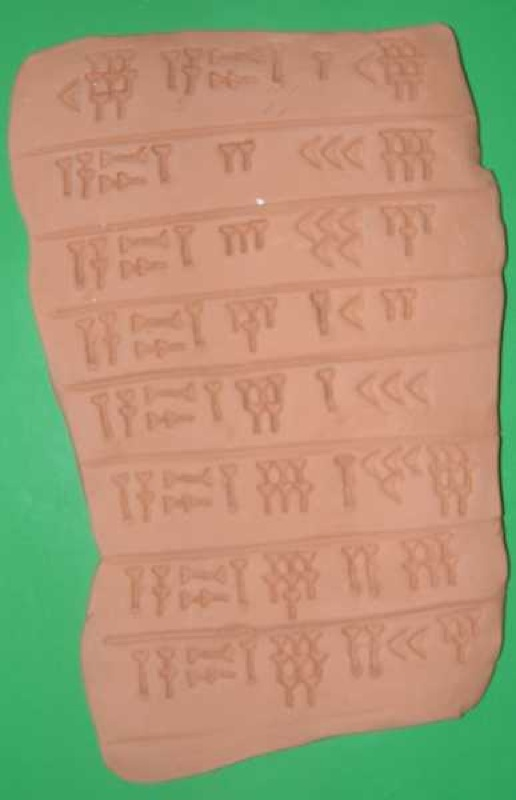
\includegraphics[height=0.3\textwidth]{pictures/babylontafel}\hspace*{0.2cm}
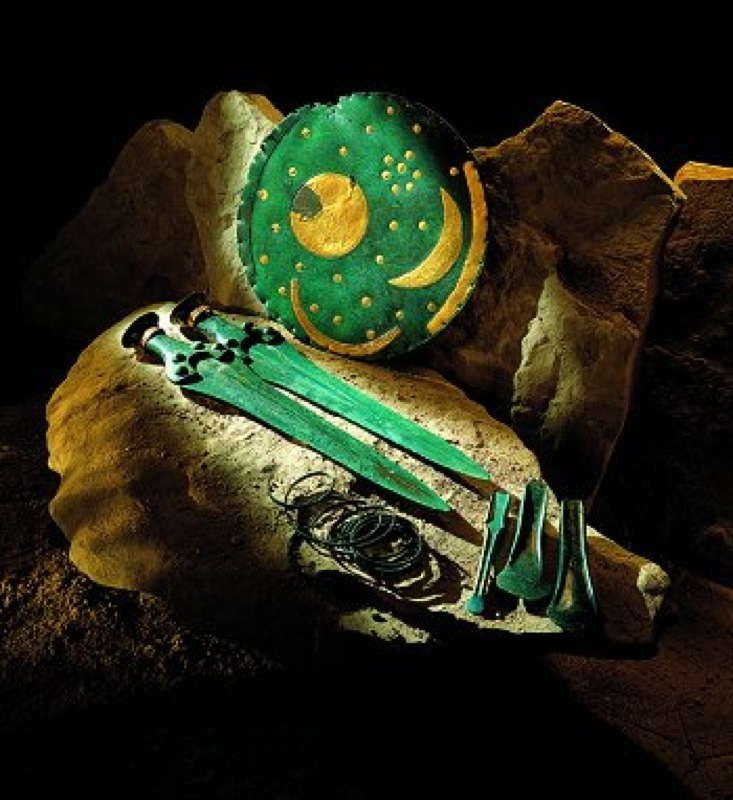
\includegraphics[height=0.3\textwidth]{pictures/babylonuhr}
\end{center}
\caption{Babylonische Rechentafel und Sternkarte}
\end{figure}
Die Babylonier verwendeten als eines der ersten Völker ein \glqq hybrides\grqq{} \textbf{Positionssystem}. Der Wert eines Zeichens hängt auch von dessen Position ab. Während wir heute in unserem Dezimalsystem (Basis $10$) die Ziffern $0, 1, 2, \dots, 9$ verwenden, brauchten die Babylonier in ihrem Sechzigersystem $59$ Ziffern. Ein Zeichen für die Null, das \glqq Nichts\grqq, gab es damals noch nicht.
\begin{ueb}
Finde eine Darstellung der Zahlzeichen der Babylonier, und schreibe das Wesentliche dieser Darstellung auf, so dass du mit deinen Notizen jede Zahl in Babylonisch schreiben kannst.
\end{ueb}

Abschliessend noch ein Beispiel, wie diese Zeichen verwendet werden.
\begin{center}
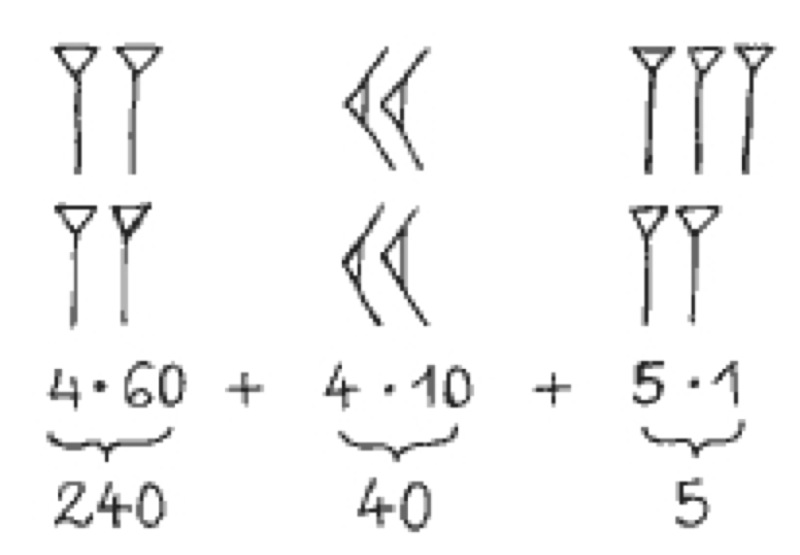
\includegraphics[width=5cm]{pictures/babylon285}
\end{center}
\begin{ueb}
Übersetze folgende Zahlen ins \glqq Babylonische\grqq:

\begin{minipage}{0.382\textwidth}
\begin{enumeratea}
\item $2381$
\end{enumeratea}
\end{minipage}
\begin{minipage}{0.23\textwidth}
\begin{enumeratea}
\addtocounter{enumi}{1}
\item $829$
\end{enumeratea}
\end{minipage}
\end{ueb}

\subsection{Zahlensysteme}
Ein Zahlensystem wird zur Darstellung von Zahlen verwendet. Eine Zahl wird dabei nach den Regeln des Zahlensystems als Folge von Ziffern dargestellt. Man unterscheidet im Wesentlichen zwischen Additionssystemen und Stellenwertsystemen (Positionssystemen).
\subsubsection{Additionssysteme}
In einem Additionssystem wird eine Zahl als Summe der Werte ihrer Ziffern dargestellt. Dabei spielt die Position der einzelnen Ziffern keine Rolle.

\subsubsection{Positionssysteme}
In einem Positionssystem bestimmt die Stelle (Position) den Wert der jeweiligen Ziffer. Die \glqq niederwertigste\grqq\ Position steht dabei im Allgemeinen rechts.

Ein Stellenwertsystem hat eine Basis $b$. Jede Zifferposition hat einen Wert, der einer Potenz der Basis entspricht. Für die $k$-te Position hat man einen Wert von $b^{k-1}$.

Die Berechnung des Zahlenwertes erfolgt durch Multiplikation der einzelnen Ziffern $z_i$ mit den zugehörigen Stellenwerten $b_i$ und Summation dieser Produkte:
$$\text{Zahlenwert} = z_n\cdot b^n+\dots+z_i\cdot b^i+\dots+z_0\cdot b^0.$$
\begin{bsp}
Unter der Zahl $1257$ im üblichen Dezimalsystem (d.h. die Basis ist $10$) verstehen wir den Wert
$$1\cdot10^3+2\cdot10^2+5\cdot10^1+7\cdot10^0 = 1257.$$
\end{bsp}

Mit der Beschränkung des niedrigsten Exponenten auf $0$ kann man nur ganze Zahlen darstellen. Lässt man auch negative Exponenten zu,
\marginnote{
\qrcode{
https://www.youtube.com/watch?v=bX32IRfefkk}
}
kann man auch rationale Zahlen in einem Stellenwertsystem schreiben, wobei der Übergang vom nichtnegativen zum negativen Exponenten durch ein Trennzeichen markiert wird, beispielsweise ein Komma:
$$1\cdot10^2+2\cdot10^1+1\cdot10^0+4\cdot10^{-1}+7\cdot10^{-2}=121,47$$

\begin{ueb}
Die Idee des Positionssystems mit einer bestimmten Basis wird auch beim Binärsystem
\marginnote{
\qrcode{
https://www.youtube.com/watch?v=y96o8U_grVE}
}
(Basis $2$) verwendet. Computer stellen Zahlen nur mit den Ziffern $0$ und $1$ dar und zwar als magnetische Polung oder elektrisches Signal (Nord oder Süd bzw. Plus oder Minus).
Die binäre Zahl $1011$ entspricht der Dezimalzahl
$$1\cdot2^3+0\cdot2^2+1\cdot2^1+1\cdot2^0=8+2+1=11.$$
Stelle die Dezimalzahlen von $1$ bis $20$ im Binärsystem dar. Beschreibe dein Vorgehen.
\end{ueb}
\begin{ueb}
Verwandle folgende Binärzahlen in Dezimalzahlen
$$1\qq11\qq111\qq1111\qq\dots$$
und
$$10\qq100\qq1000\qq10000\qq\dots$$
\end{ueb}
\begin{ueb}
Finde für die Dezimalzahl $34$ die Binärschreibweise.
\end{ueb}

\subsection{Das Binärsystem}
\subsubsection{Einleitung}
Wie könnte eine Codierung von Zeichen im Computer realisiert werden? Der Computer arbeitet mit elektrischem Strom. Das heisst er kann lediglich die beiden Zustände \glqq Strom an\grqq\ und \glqq Strom aus\grqq\ unterscheiden. Man codiert $1$ für den ersten und $0$ für den zweiten Zustand. Die Information, die durch den Strom in einer Leitung codiert ist, heisst \textbf{ein Bit} (binary digit). So lassen sich bloss zwei Zeichen codieren. Kombiniert man aber zwei Leitungen, lassen sich nun vier Zustände unterscheiden:
\begin{center}
\begin{tabular}{c|c}
Leitung 1 & Leitung 2\\ \hline
0 & 0\\
0 & 1\\
1 & 0\\
1 & 1\\
\end{tabular}
\begin{ueb}
Stelle eine Tabelle für drei Leitungen auf.
\end{ueb}
\end{center}
Dies reicht natürlich für unsere Zwecke noch nicht.
\begin{frage}
Wie viele Leitungen braucht man, um alle Buchstaben des Alphabets codieren zu können?
\end{frage}
In der Informatik ist es üblich, acht Leitungen zur Speicherung von Informationen zusammenzufassen. Insgesamt lassen sich damit $2^8=256$ verschiedene Zeichen darstellen. Man spricht bei dieser Bündelung von acht Leitungen vom Informationsgehalt ein \textbf{Byte}.
\begin{bem}
Früher rechnete man noch in Kilobyte, was ca. 1000 Bytes entspricht. Kilo wurde in diesem Zusammenhang nicht wie üblich für den Wert Tausend verwendet, sondern für $2^{10}=1024\approx1000$. Deshalb ist zum Beispiel ein Megabyte = 1024 Kilobyte.
\end{bem}
Nun zur nächsten Frage: Wie rechnet der Computer mit diesen Binärzahlen? Dabei gehen wir hier aber nicht auf die Frage ein, wie diese Rechnungen technisch realisiert werden, sondern betrachten nur die algebraischen Aspekte des Rechnens mit Binärzahlen.

\subsubsection{Rechnen im Binärsystem}
Die Addition von Binärzahlen funktioniert prinzipiell genau so, wie die Addition von Dezimalzahlen.
\begin{ueb}
Addiere schriftlich die Binärzahlen $1001011$ und $101011$.
\end{ueb}
\noindent Werden mehrere Binärzahlen addiert, kann der Übertrag natürlich auch grösser als $1$ werden.
\begin{ueb}
Addiere schriftlich die Binärzahlen $1001011$, $101011$ und $101011$.
\end{ueb}
\begin{ueb}
Berechne folgende Aufgaben, indem du alle Summanden ins Binärsystem überführst, darin addierst und das Ergebnis schliesslich ins Dezimalsystem zurück übersetzt. Kontrolliere mit der dezimalen Rechnung.
\begin{enumeratea}
\item $35+17$
\item $119+31$
\item $63+63+1$
\end{enumeratea}
\end{ueb}

\subsubsection{Negative Zahlen}
Schauen wir vierstellige Binärzahlen, sogenannte \textbf{Nibbles}, an. Insgesamt können mit einem Nibble $16$ verschiedene Zahlen dargestellt werden. Was passiert nun bei fortlaufender Addition von $1$ ausgehend von der Zahl $0$?
$$0\overset{+1}{\longrightarrow}1\overset{+1}{\longrightarrow}2\overset{+1}{\longrightarrow}\dots\overset{+1}{\longrightarrow}14\overset{+1}{\longrightarrow}15\overset{+1}{\longrightarrow}???$$
Wir können diese Additionskette als Zyklus auffassen, wenn wir die binäre Vierstelligkeit nicht verlassen wollen. Addieren wir nun zur Zahl $1111_{(2)}$ die $1$, so erhalten wir $(1)0000_{(2)}$, also die Zahl $0$ mit einem Überlauf. Wenn Addieren gleichzusetzen mit um eins im Uhrzeigersinn verschieben ist, dann sollte man Subtrahieren mit der Umkehrung definieren.
\begin{ueb}
Zeichne den Nibbles-Zyklus. Welche Binärzahl repräsentiert  $-7_{(10)}$? Addiere $-7_{(10)}+7_{(10)}$.
\end{ueb}
Die Frage, die bleibt ist: Welcher Zahl entspricht die $1000_{(2)}$? Es könnte $-8$ oder $+8$ bedeuten. Man löst dieses Dilemma, indem man einfach ein Vorzeichenbit einführt. Somit können wir also mit einem Nibble die Zahlen $-8$ bis $7$ darstellen.
\begin{ueb}
Welche Zahlen kann man analog mit einer $8$-Bit-Darstellung erzeugen?
\end{ueb}
\begin{ueb}
Suche durch Ausprobieren zur $8$-Bit-Zahl $57$ die $-57$. Hint: Notiere die schriftliche Addition mit Ergebnis $(1)00000000$.
\end{ueb}
Genau diesen Zusammenhang kann man zur Berechnung der Darstellung einer negativen Zahl im Binärsystem verwenden:
\begin{itemize}
\item Ist eine Zahl gegeben, so bildet man zuerst das sogenannte Einerkomplement, indem man einfach jedes der $8$ Bit \glqq kippt\grqq.
\item Danach addiert man noch $1$ zum Einerkomplement.
\end{itemize}
\begin{bsp}
Wir betrachten die Zahl $23=00010111_{(2)}$. Durch Kippen erhält man $11101000$. $1$ addieren bringt $11101001=-23$.
\end{bsp}
\begin{ueb}
Berechne mit Hilfe dieser Konstruktion die Binärdarstellungen von\\[2ex]
\hspace*{2.7ex} (a) $-17\q$ (b) $-118\q$ (c) $-126$
\end{ueb}
\begin{ueb}
Bestimme den Wert des Bytes $10111101_{(2)}$ im Dezimalsystem.
\end{ueb}

Wir sind nun in der Lage, die Subtraktion im Binärsystem zu lösen, indem wir sie auf die Addition zurückführen.
\begin{align*}
127-19&=127+(-19)\\
&=0111\,1111_{(2)} + 1110\,1101_{(2)}\\
&=(1)0110\,1100_{(2)}\\
&=108
\end{align*}
\begin{ueb}
Prüfe durch Rechnung obiges Beispiel. Berechne danach im Binärsystem

\begin{minipage}{0.23\textwidth}
\begin{enumeratea}
\item $115-48$
\item $77-76$
\end{enumeratea}
\end{minipage}
\begin{minipage}{0.23\textwidth}
\begin{enumeratea}
\addtocounter{enumi}{2}
\item $98-33-65$
\item $16-29$
\end{enumeratea}
\end{minipage}
\end{ueb}

\subsubsection{Multiplikation}
Neben der Addition und Subtraktion von Binärzahlen spielt die Multiplikation von Binärzahlen eine wesentliche Rolle. Wir kennen ein Verfahren in den Dezimalzahlen, welches wir direkt auf das Binärsystem anwenden können. Jedoch liegt dabei der Schwerpunkt auf dem Addieren, wie das folgende Beispiel zeigt.
\begin{bsp}
Wir berechnen das Produkt von $0000\,1001_{(2)}$ und $0010\,0111_{(2)}$. Dezimal erhalten wir $9\cdot23=207$. Binär

\begin{ueb}
Rechne!
\end{ueb}

\end{bsp}
Bei der Multiplikation entstehen so bis zu acht Summanden, die anschliessend addiert werden müssen, dagegen ist die Multiplikation sehr einfach. Ferner sieht man nun im Ergebnis zwei Bytes aneinander gereiht. Dabei haben wir Glück und das zweite Byte bleibt mit Nullen gefüllt, so dass unser Resultat wieder in ein Byte hinein passt. Es könnte ja auch sein, dass das vordere Byte benötigt wird, nämlich dann, wenn das Ergebnis grösser als $255$ ist. Man spricht beim vorderen Ergebnisbyte vom \emph{High-Byte}, beim hinteren vom \emph{Low-Byte}.

\begin{ueb}
Berechne\\[2ex]
(a) $17\cdot15\q$ (b) $7\cdot31\q$ (c) $53\cdot37$
\end{ueb}
\begin{ueb}
Vergleiche das Binärsystem mit dem Hexadezimalsystem. Beschreibe, wie man ohne grossen Rechenaufwand Zahlen im Hexadezimalsystem ins Binärsystem umwandeln kann.
\end{ueb}

\clearpage

\section{Modulo}
Modulare Arithmetik --- rechnen mit Resten --- ist ein nützliches Werkzeug der Zahlentheorie. Insbesondere kann man damit Informationen über Lösungen bestimmter Gleichungen gewinnen oder Unlösbarkeit zeigen.
\begin{figure}
  \begin{center}
    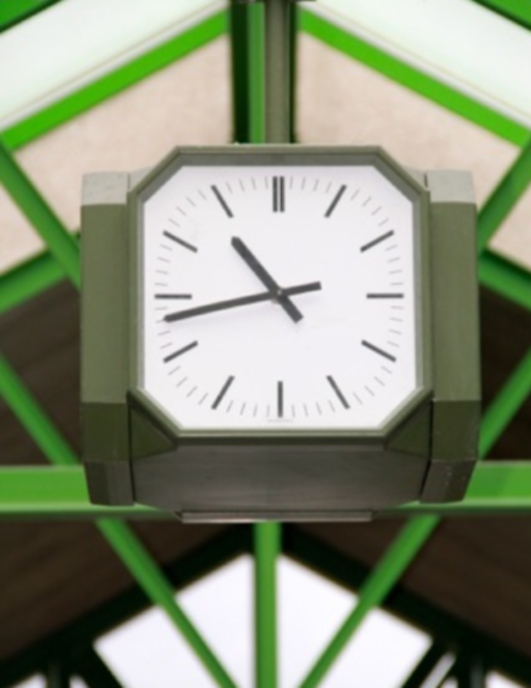
\includegraphics[width=0.3\textwidth]{pictures/uhr}
  \end{center}
%\caption{A gull}
\end{figure}

\subsection{Ein erstes Beispiel}
Wir wissen, dass die Menge $\mZ$ in zwei Klassen aufgespalten werden kann.
\begin{itemize}
\item die geraden Zahlen:
$$\dots,-6,-4,-2,0,2,4,6,\dots$$
\item die ungeraden Zahlen:
$$\dots,-5,-3,-1,1,3,5,\dots$$
\end{itemize}
Nun können wir gewisse Verallgemeinerungen über die Gesetzmässigkeiten dieser Zahlen formulieren; in Abhängigkeit ihrer Zugehörigkeit zu einer der beiden Klassen. Beispielsweise ist die Summe zweier gerader Zahlen wieder gerade. Die Summe einer geraden und einer ungeraden Zahl ist ungerade. Die Summe zweier ungeraden Zahlen ist gerade. Das Produkt zweier gerader Zahlen ist gerade, usw.

\subsection{Motivation}

Die modulare Arithmetik lässt uns diese Aussagen elegant formulieren und liefert auch eine formalisierte Sprache, um etwas komplexere Zusammenhänge einzusehen. Im obigen Beispiel ist der sogenannte \emph{Modulus} gleich $2$. Der Modulus kann als Anzahl der Klassen betrachtet werden, in die unsere Zahlenmenge $\mZ$ aufgeteilt wird. Ferner entspricht der Modulus auch der Differenz von irgend zwei aufeinander folgenden Zahlen einer Klasse.

Jetzt legen wir für jede der beiden Klassen ein Symbol fest. Wir schreiben $0$ für die Klasse aller geraden Zahlen und $1$ für die Klasse aller ungeraden Zahlen\footnote{Präziser müsste man zum Beispiel $\overline{0}$ für die Klasse der geraden Zahlen schreiben, weil $0$ ja ein Element der Klasse der geraden Zahlen ist. Falls der Kontext aber klar ist, lässt man die umständlichere Schreibweise fallen.}. Die Bezeichnung erfolgte willkürlich; wir hätten auch $2$ und $1$, oder $-32$ und $177$ wählen können. $0$ und $1$ sind aber die üblichen Bezeichnungen.
Die Aussage

\begin{quote}
Die Summe zweier gerader Zahlen ist eine gerade Zahl.
\end{quote}

wird wie folgt schlank geschrieben:
$$0+0\equiv0\mod 2$$
Hier bezeichnet das Symbol $\equiv$ nicht Gleichheit, sondern \emph{Kongruenz}. $\mod 2$ bedeutet, dass unser Modulus $2$ ist. Obige Aussage liest man: \glqq Null plus Null ist kongruent Null Modulo Zwei\grqq. Die Aussage, dass die Summe einer geraden und einer ungeraden Zahl ungerade ist, schreibt sich
$$0+1\equiv1\mod2.$$
Diese Beispiele sind trivial. Wie aber schreiben wir, dass die Summe zweier ungerader Zahlen gerade ist?
$$1+1\equiv0\mod2$$
Plötzlich sind die Symbole $\equiv$ und $\mod2$ sehr wichtig!

\noindent Analoge Aussagen erhält man für die Multiplikation:
\begin{align}
0\cdot0\equiv0\mod2\notag\\
0\cdot1\equiv0\mod2\notag\\
1\cdot1\equiv1\mod2\notag
\end{align}
Damit haben wir ein Zahlensystem mit einer Addition und einer Multiplikation kreiert, das bloss die \glqq Zahlen\grqq\  mit Ziffern $0$ und $1$ enthält.

\subsection{Definition und weitere Beispiele}

Selbverständlich kann man auch Modulo $m$, $m\in\mN$, rechnen. Wir definieren

\begin{cdef}[Modulo]{}
Sei $m\in\mN$. Zwei Zahlen $a,b\in\mZ$ heissen \emph{kongruent Modulo $m$}, falls eine $k\in\mZ$ existiert, so dass $a-b=k\cdot m$. Man schreibt
$$a\equiv b\mod m.$$
\end{cdef}

\begin{bsp}
$5$ und $8$ sind kongruent Modulo $3$, denn es gilt $5-8=-1\cdot 3$.
\end{bsp}

\begin{bem}
Die Bedingung $a-b=km$ für ein $k\in\mZ$ ist äquivalent zu $m$ teilt $a-b$.
\end{bem}

Wir betrachten ganze Zahlen Modulo $3$. Klar ist, dass alle Vielfachen von $3$, $3n$, kongruent Modulo $3$ sind, da jede Differenz zweier solcher Zahlen durch $3$ teilbar ist. Analog sind alle Zahlen der Form $3n+1$ und alle Zahlen der Form $3n+2$ kongruent Modulo $3$, $n\in\mZ$.
\begin{align}
\dots\equiv-6\equiv-3\equiv0\equiv3\equiv6\equiv9\dots\mod3\notag\\
\dots\equiv-7\equiv-4\equiv-1\equiv2\equiv5\equiv8\dots\mod3\notag\\
\dots\equiv-8\equiv-5\equiv-2\equiv1\equiv4\equiv7\dots\mod3\notag
\end{align}
Wie steht es mit $m=1$? Da jede Differenz von zwei Zahlen durch $1$ teilbar ist, ist dieser Fall nicht besonders interessant.

\subsection{Die Uhr}

Ein alltäglicher Fall ist der Modulus $12$, und er gibt uns ein leicht verständliches Schema, um Modulare Arithmetik zu verstehen. Man nennt den Fall $m=12$ auch die \glqq Uhr-Arithmetik\grqq.

\begin{bsp}
Wenn es 07:00 Uhr ist, welche Zeit haben wir in $\unit[25]{Stunden}$. Da $25\equiv1\mod12$ können wir einfach $1$ zu $7$ addieren:
$$7+25\equiv7+1\equiv8\mod12.$$
Also 08:00 Uhr. Dies ist formal der Vorgang, der sich in unseren Köpfen abspielt, wenn wir obige Frage beantworten. Die $12$ Ziffern $1$ bis $12$ repräsentieren die Uhrzeit (manchmal verwendet man auch $12=0$ um zwischen Mittag und Mitternacht zu unterscheiden). Man hat also die Klassen
$$12n,12n+1,12n+2,\dots,12n+10,12n+11$$
Die Sekunden und Minuten auf der Uhr sind auch modular, nämlich Modulo $60$.
\end{bsp}

\subsection{Rechenregeln}

Die Grundlage für folgende Rechenregeln ($a,b\in\mZ$ und $m,n\in\mN$) mit Moduln bildet

\begin{csatz}[Modulare Aequivalenz]{}
$$
a\equiv b\mod m \q\Leftrightarrow\phantom{:}\q a-b\equiv 0\mod m\Leftrightarrow:\q m\,|\,(a-b)
$$
\end{csatz}
\noindent Die restlichen Sätze, inklusive die Äqui\-valenz\-eigen\-schaf\-ten, folgen unmittelbar.
\begin{csatz}[Additon mod]{}
$$a\equiv b\mod m \q\Rightarrow\q a+c\equiv b+c\mod m$$
\end{csatz}
\begin{csatz}[Multiplikation mod]{}
$$a\equiv b\mod m \q\Rightarrow\q ac\equiv bc\mod m$$
\end{csatz}
\begin{csatz}[Potenz mod]{}
$$a\equiv b\mod m \q\Rightarrow\q a^n\equiv b^n\mod m$$
\end{csatz}
\begin{csatz}[Additivität mod]{}
$$
a\equiv b\mod m \text{ und } c\equiv d\mod m\q\Rightarrow\q a+c\equiv b+d\mod m
$$
\end{csatz}
\begin{csatz}[Multiplikativität mod]{}
$$
a\equiv b\mod m \text{ und } c\equiv d\mod m\q\Rightarrow\q ac\equiv bd\mod m
$$
\end{csatz}
\begin{csatz}[Chinese mod]{}
$$
\ggT(m,n)=1, a\equiv b\mod m \text{ und } a\equiv b\mod n\q\Rightarrow\q a\equiv b\mod mn
$$
\end{csatz}
\begin{csatz}[Primzahlprodukt]{}
Ist $p$ eine Primzahl, so gilt
$$
ab\equiv 0\mod p\q\Rightarrow\q a\equiv 0\mod p\textup{ oder }b\equiv0\mod p
$$
\end{csatz}
\begin{csatz}[Kürzungssatz]{}
$$
\ggT(a,m)=1 \textup{ und } ab\equiv ac\mod m\q\Rightarrow\q b\equiv c\mod m
$$
\end{csatz}

\begin{ueb}[Modulo]
Gib konkrete Beispiele zu den Sätzen.
\end{ueb}

\subsection{Eigenschaften der Kongruenz}

Man zeigt einfach, dass für beliebige $a,b,c$ und $m\neq0$ folgende Eigenschaften erfüllt sind:
\begin{itemize}
\item $a\equiv a\mod m$ (Reflexivität)
\item Falls $a\equiv b\mod m$, dann gilt $b\equiv a\mod m$ (Symmetrie)
\item Falls $a\equiv b\mod m$ und $b\equiv c\mod m$, dann $a\equiv c\mod m$ (Transitivität)
\end{itemize}

\begin{cdef}[Äquivalenzrelation]{}
Eine Relation, die obige drei Bedingungen erfüllt, nennt man eine \textsc{Äquivalenzrelation}. Die Äquivalenzrelation $\mod m$ teilt $\mZ$ in $m$ \textsc{Äquivalenzklassen}.
\end{cdef}

Man schreibt für die Äquivalenzklasse
\marginnote{
\qrcode{
https://www.youtube.com/watch?v=USC0Nm413FE}
}
einer Zahl $a$ etwa $[a]$ oder auch $\overline{a}$, um zwischen Zahl und Klasse zu unterscheiden.

Mit dieser Notation lässt sich die Addition $\mod m$ schreiben als
$$\overline{a+b}=\overline{a}+\overline{b}.$$
Analog gilt
$$\overline{a\cdot b}=\overline{a}\cdot\overline{b}.$$

\begin{proof}[Beweis]
Übung. Setze zum Beispiel $a=k_1m+r_1$ und $b=k_2m+r_2$ und berechne Summe und Produkt.
\end{proof}

\begin{figure}
\begin{center}
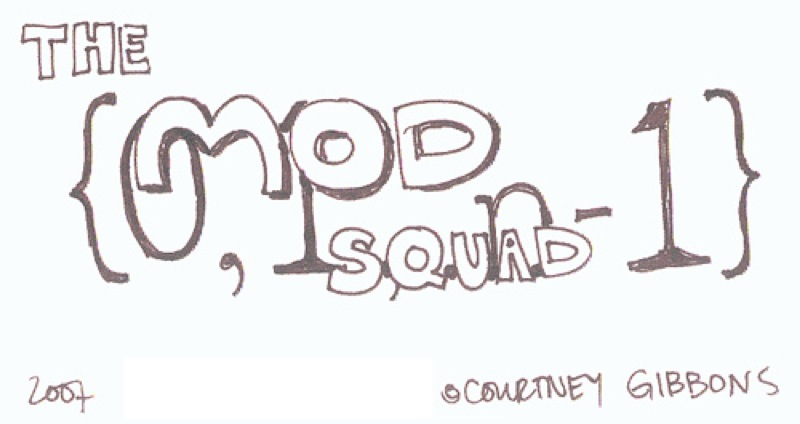
\includegraphics[width=0.618\textwidth]{pictures/modsquad}
\end{center}
\caption{The Mod Squad}
\end{figure}

\begin{ueb}[GlSys]
Zeige, dass das Gleichungssystem
\begin{align}
11x-5y=7\\
9x+10y=-3
\end{align}
keine ganzzahlige Lösung besitzt.
\end{ueb}

\begin{ueb}[GlSys schwieriger]
Zeige, dass das Gleichungssystem
\begin{align}
24x-5y=10\\
11x-9y=13
\end{align}
keine ganzzahlige Lösung besitzt.
\end{ueb}

\begin{ueb}[Pythagoras]
Zeige, dass für $x,y,z\in\mZ$ mit
$$x^2+y^2=z^2$$
mindestens eine der Zahlen durch $2$, mindestens eine durch $3$ und mindestens eine durch $5$ teilbar ist.
\end{ueb}

\begin{ueb}[Kubisch]
Zeige, dass für $x,y,z\in\mZ$ mit
$$x^3+y^3=z^3$$
mindestens eine durch $7$ teilbar ist.
\end{ueb}

\clearpage

\section{Teilbarkeit}
\subsection{Teilbarkeit durch 3}

Es gilt
\begin{csatz}[Teilbarkeit durch 3]{}
Eine
\marginnote{
\qrcode{
https://youtu.be/Vo63939DIa8}
}
Zahl ist genau dann durch $3$ teilbar, wenn es ihre Quersumme ist.
\end{csatz}
\begin{proof}[Beweis]
Sei $n\in\mN$ im Dezimalsystem als
$$n=a_ra_{r-1}\dots a_1a_0$$
geschrieben, so ist explizit
$$n=a_0+10\cdot a_1+\dots+10^r\cdot a_r.$$
Modulo $3$ ist jetzt $10\equiv1\mod3$, also $[10]=[1]$. Damit ist
\begin{align*}
[n]&=[a_0+10\cdot a_1+\dots+10^r\cdot a_r]\\
&=[a_0]+[10]\cdot[a_1]+\dots+[10]^r\cdot[a_r]\\
&=[a_0]+[a_1]+\dots+[a_r]\\
&=[a_0+a_1+\dots+a_r]
\end{align*}
das heisst, die Zahl $n$ ist Modulo $3$ gleich ihrer Quersumme. Insbesondere ist $n$ genau dann durch $3$ teilbar, wenn die Quersumme dies ist.
\end{proof}

\begin{figure}
\begin{center}
    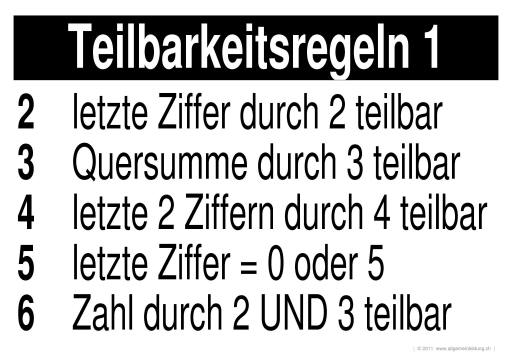
\includegraphics[width=0.382\textwidth]{pictures/regeln}
  \end{center}
%\caption{Teilbarkeit}
\end{figure}

\subsection{Teilbarkeit durch 11}

Mit der Überlegung aus dem vorigen Beispiel lässt sich rasch eine Bedingung für die Teilbarkeit einer Zahl durch $11$ herleiten. Es ist $10\equiv-1\mod11$, also ist analog zur obigen Rechnung für eine Dezimalzahl
$$n\equiv a_0-a_1+a_2-\dots+(-1)^ra_r\mod11.$$
Auf der rechten Seite steht hier die alternierende Quersumme. Eine Zahl ist also genau dann durch $11$ teilbar, wenn es ihre alternierende Quersumme ist

\begin{bsp}
$12375$ ist durch $11$ teilbar, denn
$$5-7+3-2+1=0.$$
\end{bsp}

\subsection{Teilbarkeit im Hexadezimalsystem}

\begin{ueb}[Hexa-Teilbarkeit]
Überlege dir Teilbarkeitsregeln im Hexadezimalsystem. Betrachte dazu die Teilbarkeit einer Hexadezimalzahl durch $3$, $5$ und $17$.
\end{ueb}

\section{Barcode}

Ein ähnliches System und Prüfverfahren existiert für die wohlbekannten Barcodes zum Beispiel auf Verpackungen.

\begin{figure}
\begin{center}
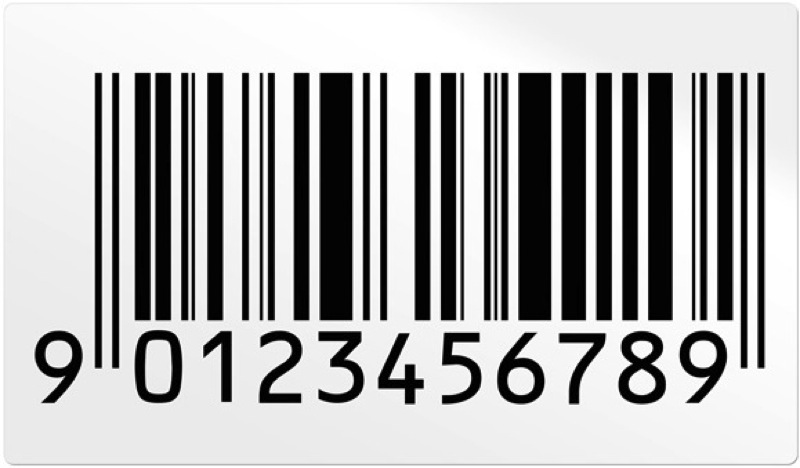
\includegraphics[width=0.5\textwidth]{pictures/barcode}
\end{center}
\caption{Barcode EAN 13}
\end{figure}

Bezahlt man in einem Geschäft seine Ware, so wird der Preis in aller Regel nicht per Hand eingegeben. Vielmehr wird der Strichcode, der sich auf jedem Artikel befindet, eingescannt; und selbst wenn dies aufgrund technischer Probleme nicht funktioniert, gibt der Kassierer nicht den Preis, sondern die zum Strichcode gehörende Ziffernfolge ein --- üblicherweise aus 13 Ziffern bestehend. Der Preis wird dann aus einer Datenbank ermittelt und in selbiger wird vermerkt, dass das Geschäft nun einen Artikel dieses Codes weniger im Sortiment hat. Wie erwähnt, manchmal funktioniert das Einscannen nicht, und eine solch lange Ziffernfolge abzutippen ist reichlich fehleranfällig. Im Falle eines Fehlers piepst die Kasse und der Kassierer gibt die Zahlenfolge noch mal ein. Wie kommt es, dass ein Fehler beim Eingeben immer auffällt?

Zunächst bedeutet es nur, dass der falsche Code nicht in der Datenbank vorkommt, was auf den ersten Blick nicht zu verwundern scheint, da der Code aus 13 Ziffern besteht. Nun werden diese Strichcodes aber nicht von den Geschäften vergeben, die die Ware verkaufen, sondern vom Hersteller --- genauer, der Hersteller lässt sie bei einer zentralen Agentur eintragen.

Der in Europa gängigste Typ des Strichcodes war bis 2008 der EAN--13, was soviel wie European Article Number der Länge 13 bedeutet. Seit 2009 heisst er GTIN für Global Trade Item Number. Vergeben werden sie von mehreren Organisationen, und die ersten zwei bis drei Ziffern des Codes identifizieren im Wesentlichen das Land. Einige der folgenden Ziffern identifizieren der Hersteller, der wiederum weitere Ziffern zur Identifikation seines Produkts zur Verfügung hat. Es kann also sein, dass sich der Code für eine $\unit[100]{g}$-Tafel Schokolade sehr wenig von dem für eine $\unit[400]{g}$-Tafel unterscheidet --- im Gegensatz zum Preis.

Man braucht also eine Idee, wie man Fehler bei der Eingabe mit hoher Wahrscheinlichkeit bemerken kann; und die Idee heisst Redundanz. Man hängt an den Teil des Codes, den man zur Identifikation des Produkts braucht, zusätzliche (redundante) Ziffern an, deren einziger Sinn es ist, den Code fehlerresistenter zu machen. Dabei sollten möglichst wenig zusätzliche Ziffern eine möglichst hohe Sicherheit bieten. Weshalb und wie man das mit nur einer Ziffer erreichen kann --- mit der sogenannten Prüfziffer --- hat mit Modulo Arithmetik und Gruppen zu tun. Ähnliche Verfahren werden auch bei Kreditkarten, ISBN-Nummern, Seriennummer von Geldscheinen etc. verwendet.

\clearpage

\section{Die alte ISBN-Nummer}
\subsection{Prüfziffern}

Als ein kleines Beispiel beschreiben wir das alte ISBN-System. Dieses ist zwar nicht mehr ganz aktuell, aber für unsere Zwecke instruktiver als die inzwischen verwendete Variante.

Jedem Buch ist eine zehnstellige ISBN-Nummer zugeordnet, die zur eindeutigen Identifikation dient. Von diesen $10$ Ziffern sind die ersten $9$ die eigentliche Information, die zehnte ist eine Prüfziffer. Diese soll eine gewisse Sicherheit zur Vermeidung von Tipp- und Übertragungsfehlern gewährleisten.
Bezeichne
$$Y=a_1a_2a_3\dots a_9a_{10}$$
eine ISBN Nummer. Dabei ist $a_i\in\set{0,1,2,\dots,9}$ und
$$a_{10}\equiv a_1+2a_2+3a_3+\dots+9a_9=\sum_{i=1}^9ia_i\mod11.$$
Dies ergibt einen Wert zwischen $0$ und $10$. Falls man $10$ erhält schreibt man ein X.

\begin{bsp}
Wir nehmen als Beispiel das Buch
\begin{quote}
P.~Hartmann, \emph{Mathematik für Informatiker}, Vieweg, 2003.
\end{quote}
mit der (alten) ISBN-Nummer 3--8348--0096--1.
\begin{frage}
Testen Sie, ob die Prüfziffer korrekt ist.
\end{frage}
\end{bsp}

\noindent Natürlich kann man nicht erwarten, dass so alle Fehler erkannt werden. Aber, wie Sie gleich sehen werden, schützt das Modul $11$ vor den alltäglichen.

\subsection{Ziffer fehlerhaft eingetippt}

Geschieht
der Fehler in der Prüfziffer selbst, dann ist der Fall klar. Wir können also den Fehler zwischen $1$ und $9$ annehmen und müssen zeigen, dass die Prüfziffer falsch ist. Sei also
$$Y'=a_1\dots a_i'\dots a_{10}$$
die fehlerhafte ISBN mit dem Fehler an der $i$-ten Stelle, $1\leq i\leq9$. Die Prüfziffer wäre so
$$a'_{10}=\sum_{j\neq i}ja_j+ia_i'\mod11$$
Wir haben aber $a_{10}$ und es gilt
$$a_{10}-a_{10}'=ia_i-ia_i'=i(a_i-a_i')\mod11$$
Wegen $a_i\neq a_i'$ ist $a_i-a_i'\neq0$ und wegen $1\leq i\leq9$ auch $i\neq0$. Daraus folgt mit einer nicht ganz trivialen Überlegung, dass $i(a_i-a_i')\not\equiv0\mod11$. Dabei ist die Wahl des Moduls wichtig. Entscheidend für die letzte Folgerung ist, dass $11$ eine Primzahl ist, denn für diese haben wir

\begin{csatz}[Primfaktorsatz]
Sind $p$ prim und $a,b\in\mZ$ mit $p|ab$, so gilt $p|a$ oder $p|b$.
\end{csatz}

Wir brauchen die Negation des obigen Satzes: Teilt $p$ weder $a$ noch $b$, dann teilt $p$ auch nicht $ab$.

\begin{proof}[Beweisskizze]
Wenn $p$ weder $a$ noch $b$ teilt, dann kommt $p$ nicht in der Primfaktorzerlegung von $a$ und $b$ vor, also auch nicht in der Primzahlzerlegung des Produkts $ab$. Das heisst $p$ teilt $ab$ nicht.
\end{proof}

Damit ist gezeigt, dass insbesondere für $p=11$ der letzte Schritt gilt und damit die Prüfziffer der ISBN eine fehlerhafte Ziffer erkennt.

\begin{bem}
All dies würde nicht funktionieren, wenn wir anstelle von $11$ beispielsweise $10$ als Modul verwendet hätten. Denn wegen $10=2\cdot5$, also $2\cdot5\equiv0\mod10$ würde etwa ein Fehler an der $i=5$-ten Stelle nicht erkannt, wenn die fehlerhafte Ziffer um $2$ von der korrekten Ziffer abweicht. Die Prüfziffer Modulo $10$ bliebe unverändert.
\end{bem}
\begin{ueb}
Bestätige zuerst für die erste, korrekte ISBN-Nummer, dass die Prüfziffer Modulo $10$ gleich $0$ ist.
\begin{itemize}
\item 3--8348--0096--0
\item 3--8346--0096--0
\end{itemize}
Zeige anschliessend, dass die zweite, vertippte Nummer dieselbe Prüfziffer ergibt und somit der Fehler nicht entdeckt wird. Schliesslich berechne man die Prüfziffer für die falsche ISBN $\mod 11$.
\end{ueb}

\begin{bem}
Wie oben gesehen, ist also die Wahl des Moduls entscheidend. Bei $9$ informationstragenden Ziffern braucht man also eine Primzahl grösser oder gleich $10$, und $11$ ist dafür die kleinstmögliche Wahl.
\end{bem}

\subsection{Zahlendreher}

Die
\marginnote{
\qrcode{
https://youtu.be/2VNHnWVAP_8}
}
ISBN erkennt nicht nur einzelne fehlerhafte Ziffern, sondern auch den am häufigsten auftauchende Fehlertyp: das Vertauschen zweier aufeinanderfolgender Ziffern. In der Tat erkennt die Prüfziffer sogar Vertauschen von nicht unmittelbar aufeinanderfolgenden Ziffern, was zwar weniger vorkommt, aber für den folgenden Beweis ohne Mehraufwand mit einbezogen werden kann.

Sei
$$Y'=a_0\dots a_{i-1}a_ja_{i+1}\dots a_{j-1}a_ia_{j+1}\dots a_{10}$$
eine falsche ISBN, die durch Vertauschen der $i$-ten mit der $j$-ten Ziffer entstand, $1\leq i<j\leq9$. Zwei Fälle lassen wir aussen vor. Erstens, dass die Prüfziffer eine der vertauschten Ziffern ist (diesen Fall könnte man separat behandeln), und zweitens, dass die vertauschten Ziffern identisch sind, dann hätte ja der Verdreher keine Wirkung. Als Prüfziffer für $Y'$ erhält man so
$$a_{10}'\equiv\sum_{k\neq i,j}ka_k+ia_j+ja_i\mod11,$$
also
\begin{align*}
a_{10}-a_{10}'&=ia_i+ja_j-ia_j-ja_i\\
&=i(a_i-a_j)-j(a_i-a_j)\\
&=(i-j)(a_i-a_j).
\end{align*}
Wegen $-8\leq i-j<0$ und $0<\abs{a_i-a_j}\leq9$ gilt wiederum $i-j\not\equiv0\mod11$ und $a_i-a_j\not\equiv0\mod11$. Daraus folgt analog zur fehlerhaften Ziffer $a_{10}-a_{10}'\not\equiv0$. Die Prüfziffer ist also fehlerhaft, und der Zahlendreher wird erkannt.

\begin{ueb}[Zahlendreher]
Teste einen Zahlendreher anhand von 3--8348--0069--0.
\end{ueb}

\clearpage

\clearpage

\section{Rechnen Modulo 17}

Nimmt
\marginnote{
\qrcode{
https://youtu.be/TzfQ49a8FIM}
}
man für das Modul eine Primzahl, so hat man eine Reihe von interessanten Besonderheiten. Wir nehmen als Primzahl $17$. Man rechnet Modulo $17$ wie üblich. So ist beispielsweise $13+8=21\equiv 4\mod 17$ oder $4-9=-5\equiv12\mod17$. Ferner $5\cdot4=20\equiv3\mod17$ und $9\cdot 2=18\equiv1\mod17$. Die letzte Kongruenz besagt, dass $9$ dasselbe ist wie $\frac{1}{2}$ (Modulo $17$).

\subsection{Potenzen}
Wir berechnen illustrativ alle Potenzen von $3$ Modulo $17$.

\begin{ueb}
Vervollständige folgende Tabelle\\

\begin{center}
\Large
\begin{tabular}{|c|c|c|c|c|c|c|c|c|c|c|c|c|c|c|}
\hline
n & 0 & 1 & 2&3&4&5&6&7\\
\hline
$3^n$&1&3&9&10& & & & \\
\hline\hline
n&8&9&10&11&12&13&14&15\\
\hline
$3^n$& & & & & & & &\\
\hline
\end{tabular}
\end{center}
\normalsize
\end{ueb}

\noindent Es fällt auf, dass jede Zahl ungleich $0$ eine Potenz von $3$ ist, also jeder mögliche, nichttriviale Rest taucht genau einmal auf. Ausserdem stellt man fest, dass
$$3^{16}\equiv3\cdot6=18\equiv1\mod17.$$
Die Tatsache, dass alle Zahlen ausser $0$ eine Potenz von $3$ sind und ausserdem $3^{16}\equiv1\mod17$, hat zur Folge, dass jede Zahl $a\not\equiv0\mod17$ als $16$-te Potenz den Wert $1$ hat. Denn $a$ ist eine Potenz von $3$, also $a=3^n$ und daher
$$a^{16}=(3^n)^{16}=(3^{16})^n\equiv1^n=1\mod17$$
Das bedeutet, es gilt auch
$$a^{17}=a, a^{33}=a, a^{49}=a, \dots$$
und daraus erhält man
$$a=a^{33}=a^{3\cdot11}=(a^3)^{11}.$$

\begin{bem}
Man zieht die dritte Wurzel, indem man mit $11$ potenziert.
\end{bem}

\begin{ueb}[Wurzeln]
Ziehe durch Potenzieren
\begin{enumeratea}
\item die siebte Wurzel aus $a^7\mod17$
\item die fünfte Wurzel aus $a^5\mod17$
\end{enumeratea}
\end{ueb}

\subsection{Kryptographie --- eine erste Idee}

Diese letztgenannten Beziehungen enthalten eine der Grundideen zur Verschlüsselung mittels Zahlentheorie. Benutzt man die $16$ Zahlen von $1$ bis $16$ als (verkürztes) Alphabet, so kann man die Potenzierung mit $3$ als Verschlüsselung und die Potenzierung mit $11$ als Entschlüsselung benutzen.

\begin{bsp}
Es gilt $a^{33}\equiv a\mod17$. Wir wählen den Buchstaben c, den dritten im Alphabet, und verschlüsseln ihn durch $3^3\equiv10\mod17$, was einem K Ciphertext entspricht. Wir entschlüsseln durch $10^{11}\equiv3\mod17$ und haben wieder den Klartext c.
\end{bsp}

Ein besonders angenehmer Aspekt dieses Verfahrens ist, dass man zur Ver- und Entschlüsselung dasselbe Verfahren benutzen (Potenzierung) und dass die Reihenfolge von Ver- und Entschlüsselung vertauscht werden kann. Dies eröffnet interessante Möglichkeiten in der Kryptographie. Die Anwendbarkeit des Verfahrens hängt nun entscheidend davon ab, ob und wie leicht man zum Verschlüsselungsexponenten $3$ den Entschlüsselungsexponenten $11$ ermitteln kann. Um Analysen von Verschlüsselungsmethoden zu erstellen und Aussagen über die Sicherheit einer Methode machen zu können, muss man sich gut in Modularer Arithmetik auskennen.

\clearpage

\appendix

\begin{multicols}{2}
[
\section{Die schwere Geburt der Null}\label{ap:null}
Die Null wurde lange nach den anderen Zahlen erfunden. Die R\"omer kannten sie überhaupt nicht, die Babylonier konnten nicht mit ihr umgehen, erst die Inder erkannten das Potential dieser bizarren Zahl, die alleine nichts ist, aber anderen zur Gr\"osse verhelfen kann.
]
Die Hälfte der elektronischen Datenverarbeitung und damit ein grosser Teil unseres modernen Lebens besteht aus Nullen. Das Darstellen des Alphabets und der Ziffern als Kombinationen von 0 und 1 hat sich für den geistig beschränkten Computer als am besten erwiesen: Das simple Ja oder Nein des binären Zahlensystems kann die Maschine ohne viel Werweissen verdauen. Dass dabei selbst ein kurzer Text zum fast endlosen Wurm aus Nullen und Einsen wird, kompensiert der Rechner mit Arbeitswut.
\\
Dem Laien ist die in der Maschinensprache verborgene digitale Omnipräsenz der Null nicht bewusst. Die Null begegnet uns im Alltag jedoch auch unverhüllt. Da kostet eine Eigentumswohnung 630 000 Franken; für 7 500 000 Euro wird in Brüssel ein griechisches Strassenprojekt gesprochen. Ein Kraftwerk leistet 1 200 000 000 Watt; das im Elektronenmikroskop sichtbar gemachte Virus ist 0,000000025 Meter lang. Durch Eindampfen von beispielsweise neun Nullen zu 'Giga' oder 'Nano' lässt sich das Gewusel immerhin lesbarer machen.
\\
Dass ein Übermass an Nullen schaden kann, zeigt der in den zwanziger Jahren des letzten Jahrhunderts in Deutschland diagnostizierte 'Null-Anfall', eine Krankheit, die während der Hyperinflation auftrat: Die Notwendigkeit, beim Bäcker für ein Brot Hunderte von Milliarden Mark hinzublättern und Briefmarken mit Heerscharen von Nullen aufzukleben, liess etliche Bürger die psychische Balance verlieren. Als häufiges Symptom zeigte sich bei den 'Null-Kranken' ein Zwang, endlose Reihen von Nullen zu schreiben.
\\
Bei massvollem Gebrauch empfinden wir die Null indes als durchaus anständiges Mitglied der Ziffernfamilie. Dabei ist die Null alles andere als gewöhnlich. Schon die einfachsten Rechenoperationen enthüllen ihr bizarres Wesen. Addiert man zu irgendeiner Zahl null oder subtrahiert man sie davon, ändert sich überhaupt nichts. Wehe aber, man multipliziert mit null. Jetzt geht jede noch so stolze Zahl mit einem Schlag zugrunde und wird selber zur Null.
\\
Und wem es einfallen sollte, eine Zahl durch null zu dividieren, wird von der Mathematikerzunft als verrückt erklärt. Denn das Resultat der Division durch null müsste eine Zahl sein, die, mit null multipliziert, wiederum die Ausgangszahl ergibt. Da aber jede noch so exotische Zahl mit null multipliziert immer nur null und niemals eine von null verschiedene Zahl liefern kann, haben die Mathematiker das Teilen durch null kurzerhand verboten. Ein Gewitzter mag einwenden, man könnte doch wenigstens das Teilen von null durch null erlauben, denn dann gebe es als Lösung beispielsweise die Zahl 23, die mit null multipliziert tatsächlich zur Ausgangszahl Null zurückführt. 'Gut und recht, aber mathematisch trotzdem unanständig', erwidert der Zahlenmann. Denn da jede Zahl mit null multipliziert null ergibt, brächte ein erlaubtes Teilen von null durch null als Lösung den gesamten Zahlenkosmos - eine Beliebigkeit, die für den rechtschaffenen Mathematiker wohl noch schlimmer ist als das Fehlen einer Lösung.
\\
Die Null kann also als Rechenpartner wirkungslos wie auch zerstörerisch sein und Unmögliches oder Beliebiges hervorbringen. Zur Venus mit fast grenzenloser Fruchtbarkeit wird das leere Rund, wenn man es ans Ende einer Zahl hängt. Aus 37 wird 370 und bald schon 370 000 000 000. Die Eigenschaft, an und für sich zwar wertlos zu sein, durch das Auftauchen an einem bestimmten Platz aber aus einer bescheidenen Zahl eine respektable Grösse und sogar einen Giganten zu machen, ist die wohl grösste Tugend der Null.
\\
So selbstverständlich solcher rechnerische Nutzen uns heute erscheinen mag - der Weg der Null in die Welt war alles andere als leicht. Nicht nur bereitete ein Rechnen mit dem 'Nichts' philosophische Sorgen, das wechselhafte Gesicht der Null weckte mancherorts Misstrauen. So verlangt auch noch im dritten Jahrtausend nach Christus meine Bank, dass ich die 5030 Franken auf dem Check zusätzlich als 'fünftausendunddreissig' ausschreibe.
\\[5mm]
Eine Vorläuferin der Null schufen die babylonischen Mathematiker. Hier kannte man schon zu Beginn des 2. Jahrtausends v. Chr. eine Zahlenschrift aus Ziffern, deren Wert von der Position innerhalb der dargestellten Zahl abhing. Eine Konvention, die wir auch aus unserm Zehnersystem kennen, wo 324 selbstverständlich 3 Hunderter, 2 Zehner und 4 Einer bedeutet - und nicht etwa 3 plus 2 plus 4, also 9. Dass dies keineswegs so sein muss, zeigte die römische Zahlenwelt, die 3 Hunderter mit CCC, 2 Zehner mit XX und 4 Einer mit IV darstellte. Römisch C bedeutete also immer 100, wo immer das Zeichen in der Zahl auftauchte. Für grosse Zahlen wurde das römische Zahlensystem aber schwerfällig. So behalf man sich mit Zusatzzeichen, indem etwa ein waagrechter Strich über der Zahl das Tausendfache und ein unten offener Rahmen um die Zahl herum das Hunderttausendfache bedeuteten.
\\
Die Babylonier kamen mit lediglich zwei Ziffern aus: Ein senkrechter Nagel bedeutete eins; ein nach rechts offener Winkel stand für die Zehn. So kombinierte man bis zu 5 Winkel mit bis zu 9 Nägeln und kam damit auf 59. Wollte man 60 schreiben, schrieb man wieder einen einzigen Nagel und meinte damit einen 'Sechziger'. Und hatte man mit 5 Winkeln und 9 Nägeln 59 Sechziger beisammen, kam für die Zahl 3600 (60 mal 60) wiederum der einzelne Nagel zum Zug. Damit hatten die Babylonier ein Positionssystem erfunden, welches den Ziffern je nach Stellung innerhalb der Zahl eine bestimmte Ordnung gab: von rechts her als 1. Ordnung die Einer, als 2. die Sechziger, als 3. Ordnung die Sechzigmalsechziger usw.
\\
Ein solches Sechzigersystem anstelle des uns vertrauten Zehnersystems mag befremden. Aber auch wir pflegen das babylonische Erbe, wenn wir 5 Stunden, 32 Minuten und 19 Sekunden schreiben - insgesamt 19 939 Sekunden, dargestellt als 1., 2. und 3. Ordnung im Sechzigersystem. Und auch beim Winkelmessen geben wir uns babylonisch.
\\
Hatte nun ein babylonischer Händler 62 zu schreiben, ritzte er für 60 einen Nagel in den weichen Ton der Schreibtafel und rechts davon nochmals zwei Nägel für 2. Um zu zeigen, was 60 war und was 2, liess er zwischen dem ersten und den beiden andern Nägeln eine kleine Lücke. Falls er aber 3602 meinte, musste der Abstand noch breiter sein, denn jetzt war deutlich zu machen, dass es keinen Sechziger gab und der erste Nagel ganz links vielmehr 60 mal 60 bedeutete.
\\
Das Missverständnis war programmiert. Zerstreute oder nachlässige Schreiber vergassen oftmals einen Zwischenraum. Und wenn man zwei oder mehrere fehlende Ordnungen mit entsprechend breiter Lücke zu markieren hatte, waren Fehlinterpretationen fast unvermeidlich. Die babylonischen Gelehrten begegneten Unklarheiten mit zusätzlichen Kommentaren oder erkannten die Grössenordnung der Zahl aus dem Kontext heraus. Dies war im Sechzigersystem dank dem relativ grossen Sprung von einer Ordnung zur nächsten einfach. Denn dass der Bauer für das Tempelfest eher 5 als 5 mal 60 Schafe spendierte, war dem klerikalen Buchhalter klar.
\\[5mm]
Es dauerte fast weitere 2000 Jahre, bis ein unbekannter heller Kopf im Zweistromland auf den Gedanken kam, man könne doch das Fehlen einer Ordnung innerhalb der Zahl mit einem speziellen Zeichen markieren: Auf einer astronomischen Tafel aus Uruk stehen dort, wo zwischen dem 2 mal 3600 der 3. Ordnung und dem 15 der 1. Ordnung eine 2. Ordnung fehlt, als Platzhalter zwei schräg hochgestellte kleine Nägel, ähnlich einem Apostroph. Damit war eindeutig klar, dass 7215 (2 mal 3600 plus 15) und nicht etwa 135 (2 mal 60 plus 15) gemeint war - Babylon hatte die 'Null' erfunden. Die Tafel mit der Urnull gehört heute zur Sammlung des Louvre in Paris.
\\
Nun gab es mit der Null ein Symbol für die Leerstelle, eine Marke für eine fehlende Ordnung innerhalb der Zahl. Diese frühe Null verstanden die Mathematiker aber noch keineswegs als leere Menge oder als 'Zahl Null', mit der sich auch rechnen liesse. So war der babylonische Buchhalter nach wie vor ratlos, wenn er zwei gleich grosse Mengen voneinander zu subtrahieren hatte. Und er notierte: '20 minus 20 . . . du weisst ja.' Ein anderer Schreiber zog sich mit der Bemerkung 'Das Korn ist ausgegangen' aus der Affäre, als bei der Abrechnung einer Getreideverteilung das Ergebnis null geworden war.
\\[5mm]
Die Null in ihrem ganzen mathematischen Reichtum schenkte Indien der Welt. In Nordindien entwickelten die Gelehrten im dritten Jahrhundert v. Chr. ein Zehnersystem, wobei man für die Ziffern 1 bis 9 abstrakte, graphische Zeichen schuf. Darin sind bereits unsere modernen Grundziffern zu erkennen. Unsere Ziffern heissen deshalb zu Unrecht 'arabisch'. Die Araber hatten lediglich als Handelspartner der Inder deren Zahlensystem und Algebra kennen- und schätzengelernt und schliesslich ans christliche Abendland weitervermittelt. Allerdings reicherten die Araber das indische Wissen mit zahlreichen eigenen Erkenntnissen an; mit seinen Büchern über die indische Mathematik wurde Mohammed Ibn Musa al-Charismi um 800 n. Chr. zum Wegbereiter moderner Mathematik in Europa. Der Name des Autors wurde als alchoarismi und später algorithmus zum Synonym für das neue Rechnen.
\\
Die Inder schufen für die Ziffern 1 bis 9 verschiedene Serien von Zeichen, je nachdem, ob sie Einer, Zehner, Hunderter, Tausender oder Zehntausender bezeichneten. Damit liessen sich Zahlen bis 99 999 darstellen - für die Astronomen mit ihrer Leidenschaft für grosse Zahlen nicht genug. Die Himmelsgucker griffen deshalb auf das Sanskrit, die Sprache der Gelehrten, zurück. Sie gaben den Grundziffern Namen (1, 2, 3, 4 . . . eka, dvi, tri, catur . . .), ordneten den Zehnerpotenzen ebenfalls Sanskritwörter zu (10, 100, 1000 . . . dasa, sata, sahasra . . .) und erweiterten mit Begriffen für sehr hohe Potenzen (etwa padma für 1 000 000 000) das Zahlensystem fast beliebig.
\\
Eine Zahl wurde nun durch simples Aneinanderreihen der Namen, beginnend mit der kleinsten Ordnung, ausgedrückt: dvi eka sata ca tri sahasra (zwei, einhundert und dreitausend). Im 5. Jahrhundert n. Chr. hatten die indischen Mathematiker die geniale Idee, ihr Zahlensystem stark zu vereinfachen, indem sie fortan auf ein Erwähnen der Potenzen verzichteten. Dies konnte aber nur funktionieren, falls man fehlende Potenzen mit einem eigenen Wort anzeigte. Mit sunya für 'Leere' schufen die Inder ihre mathematische Null. Mit dvi sunya eka tri waren nun zwei Einer, kein Zehner, ein Hunderter und drei Tausender gemeint, also 3102. Damit hatten die Zahlenfreunde am Ganges sowohl ein Positionssystem als auch die Null erfunden - ein Fortschritt, der mit dem Buddhismus und dem Gewürz- und Elfenbeinhandel rasch nach Kambodscha zu den Khmer und bis nach Java getragen wurde.
\\
Die Gelehrten Indiens liebten die Dichtkunst, und Astronomen kleideten ihre Zahlen in prachtvolle Versform. Für das Auswendiglernen nummerischer oder astronomischer Tabellen mag den Gelehrten der Rhythmus von Worten und Versen zwar nützlich gewesen sein, rechnen aber liess sich mit den Gedichten beim besten Willen nicht. So benutzte der indische Händler für das profane mathematische Tun den Abakus, das Rechenbrett. Dabei wurden Kieselsteine oder Marken in Kolonnen angeordnet und entsprechend den vier Grundrechenarten verschoben. War in einer Kolonne der Zehner, Hunderter usw. voll, erfolgte ein Übertrag zur nächsthöheren Kolonne. Dass sich damit auch mit grösseren Zahlen flink rechnen lässt, kann man noch immer im Fernen Osten oder in Russland bewundern.
\\
Die Inder verwendeten als Abakus ein mit feinem Sand bestreutes Brett. Zur Abgrenzung der Kolonnen zog man senkrechte Linien, als Ziffern schrieb man 1 bis 9 in den Sand. Beim Rechnen wischte man dann laufend die alten Ziffern weg und schrieb das neue Ergebnis zwischen die Linien. Und wurde eine der Kolonnen null, blieb der Platz einfach leer.
\\
Zu Beginn des 6. Jahrhunderts n. Chr. kamen in Nordindien die Kaufleute auf die Idee, das Grundkonzept der Zahlenlyrik der Gelehrten - das Positionssystem und die Null - für das tägliche Geschäft zu nutzen. Man verzichtete beim Abakus auf die Spalten und gab den Ziffern je nach Position innerhalb der Zahlendarstellung die entsprechende Zehnerpotenz. Und wo 'Leere' zu markieren war, schrieb man einen Punkt und später einen kleinen Kreis: die Ziffer Null, wie wir sie noch heute kennen, war geboren. Die Schönheit der neuen Ziffer entzückte wiederum den Poeten, und Biharilal schrieb an eine Frau: 'Der Punkt auf Ihrer Stirn vermehrt Ihre Schönheit zehnfach - wie der Null-Punkt eine Zahl verzehnfacht.'
\\
So weit waren im Prinzip schon die Babylonier gekommen. Aber während man sich in Mesopotamien fortan auf den Gebrauch der Null als Platzhalter innerhalb der Zahlendarstellung beschränkte, erkannten die Inder rasch das enorme Potential der Null als Zahl und leere Menge. Schon 628 n. Chr. präsentierte der Astronom Brahmagupta in seinem mathematischen Werk, wie man die fünf Grundoperationen Addition, Subtraktion, Multiplikation, Division und Potenzierung nicht nur auf 'Güter' (positive Zahlen), sondern auch auf 'Schulden' (negative Zahlen) und auf 'das Nichts' (die Zahl Null) anwendet. So wurde, in strenger Logik, etwa eine Schuld, abgezogen vom Nichts, zum Guthaben oder ein Guthaben, abgezogen vom Nichts, zur Schuld. In kosmischer Grosszügigkeit wagte sich Brahmagupta sogar an das Teilen durch Null: 'Dividiert man irgendeine Zahl durch das Nichts, wird Unendlichkeit.' Damit hatte Indien der Welt die Algebra geschenkt. Der Weg für weitere Verallgemeinerungen des Zahlbegriffs war frei; Naturwissenschaft und Technik hatten eine solide mathematische Basis. Wer nun glaubt, die östliche Weisheit sei in der Alten Welt freudig begrüsst worden, kennt die mittelalterlichen Köpfe nicht. Zwar lernte der französische Mönch Gerbert d’Aurillac um das Jahr 970 auf einem Bildungsurlaub in Andalusien von arabischen Lehrmeistern die indische Zahlenschrift und das entsprechende Rechnen. Beim Versuch aber, die geniale Methode auch im christlichen Europa einzuführen, stiess der Kleriker auf geschlossenen Widerstand. Zwar akzeptierte man auf dem Abakus anstelle der einzelnen Kieselsteine Rechenmarken aus Horn mit den 'arabischen' Ziffern 1 bis 9. Doch von der Null oder einem Rechnen damit wollte man nichts wissen. Erzkonservative setzten auf die neuen Hornplättchen lieber die römischen Ziffern I bis IX, um ja nicht mit den 'teuflischen Zeichen der Araber' in Berührung zu kommen.
\\
Erst der Mathematiker Leonardo Fibonacci aus Pisa, der schon als Schulkind mit seinem handeltreibenden Vater ins muslimische Nordafrika gereist war, überzeugte im 13. Jahrhundert die Kaufleute vom grossen Nutzen der indoarabischen Rechenkunst. Denn mit den negativen Zahlen und der Null liessen sich in den Büchern endlich auch Schulden und Verluste mathematisch sauber aufrechnen. In Florenz allerdings traute man der Sache weiterhin nicht. Per Gesetz wurde 1299 kurzerhand das Verwenden arabischer Zahlen in Verträgen und offiziellen Dokumenten verboten. Die Massnahme hatte immerhin einen handfesten Grund: In der Zeit vor der Erfindung der Druckkunst war die Angst vor Fälschungen gross. So praktisch arabische Ziffern zum Rechnen waren, an die Zahl liess sich leicht eine weitere Ziffer hängen, oder Fälscher machten hurtig eine 6 oder 9 aus der 0.
\\
Es war ebenfalls Fibonacci, der aus dem arabischen Wort as-sifr (die Leere) den lateinischen Namen zefirum kreierte, woraus sich schliesslich zero entwickelte. Aus as-sifr entstand auch das lateinische cifra und später das französische chiffre und unsere Ziffer, wobei man den ursprünglichen Begriff für null generell auf alle arabischen Ziffern ausdehnte.
\\[5mm]
So nützlich die indisch-arabische Mathematik für Europas Kaufleute gewesen sein mag, ihrer breiten Einführung setzte sich nicht zuletzt die Kirche entgegen. Denn der Algorithmus, das Schreiben arabischer Ziffern mit der Feder, war selbst vom einfachen Volk erlernbar, während der Umgang mit dem Abakus doch eher dem Berufsrechner, oft ein Geistlicher, vorbehalten war. Während Jahrhunderten tobte zwischen den 'Algoristen' und den 'Abakisten' ein ideologischer Kampf. Den definitiven Durchbruch schaffte die indische Erfindung erst mit der Französischen Revolution, als mit der Verbannung des Abakus aus Schule und Verwaltung endlich der Weg für die 'demokratische' Arithmetik frei wurde.
\end{multicols}

\section{Die Osterformel von Gauss}

Die Gauss'sche Osterformel
\marginnote{
\qrcode{
https://youtu.be/7j-igVTq7l0}
}
erlaubt die Berechnung des Osterdatums für ein gegebenes Jahr. Das Verfahren gilt allgemein für den Gregorianischen Kalender.

\begin{bem}
In seltenen Fällen kann der Algorithmus im Gregorianischen Kalender den 26. April als spätesten Ostersonntag liefern. Die bei der Kalenderreform aufgestellte Zusatzbestimmung, dass der letzte mögliche Ostersonntag der 25. April ist, muss zusätzlich beachtet werden.
\end{bem}

Nun zum Verfahren ($\divis$ steht für eine ganzzahlige Division ohne Nachkommastellen):
\begin{align*}
a &= \text{Jahr}\mod19\\
b &= \text{Jahr}\mod4\\
c &= \text{Jahr}\mod7\\
k &= \text{Jahr}\divis100\\
p &= (8k+13)\divis25\\
q &= k\divis4\\
M &= (15+k-p-q)\mod30\\
N &= (4+k-q)\mod7\\
d &= (19a+M)\mod30\\
e &= (2b+4c+6d+N)\mod7
\end{align*}
Mit den so bestimmten Variablen kann man nun das Osterdatum berechnen:
$$\text{Ostern}=(22+d+e)\text{ter März},$$
wobei der 32. März der 1. April ist etc.

\begin{ueb}[Gauss'sche Osterformel]
Berechne das Datum der nächsten Ostern.
\end{ueb}

\section{Abschliessende Übungen}

\begin{ueb}[Teilbarkeit durch $7$]
Ist
$$222^{555}+555^{222}$$
durch $7$ teilbar?
\end{ueb}

\begin{ueb}[Äquivalenz]
Für welche Modul $m\in\mN$ gilt $[\,7\,]=[\,1\,]$?
\end{ueb}

\begin{ueb}[variabel]
Zeige, dass für $a,b\in\mN$ gilt: Ist $100a+b$ durch $7$ teilbar, dann ist es auch $a+4b$.
\end{ueb}

\begin{ueb}[Gleichungen]
Löse die Gleichungen Modulo $7$:

\begin{minipage}{3.5cm}
\begin{enumeratea}
\item $x^2=1$
\item $x^6=1$
\end{enumeratea}
\end{minipage}
\begin{minipage}{3.5cm}
\begin{enumeratea}
\addtocounter{enumi}{2}
\item $3x+5=1$
\item $2x-1=15$
\end{enumeratea}
\end{minipage}
\end{ueb}

\begin{ueb}[natürliche Nachfolger]
Zeige, dass unter $n$ aufeinanderfolgenden natürlichen Zahlen stets genau eine gibt, die durch $n$ teilbar ist.
\end{ueb}

\begin{ueb}[prim hoch 2]
Zeige, dass für jedes $p>3$ prim $(p^2-1)$ durch $24$ teilbar ist.
\footnotesize \\Hint: Zeige, dass $2,3$ und $4$ in der Faktorzerlegung von $p^2-1$ vorkommen.
\end{ueb}

\cleardoublepage
\listoffigures
%\listoftables
%\newpage
%\nocite{*}
%\bibliographystyle{plain}
%\bibliography{preamble/literaturgoogle}
\end{document}